
%----------------------------------------------------------------------------------------
%	PREAMBUŁA
%----------------------------------------------------------------------------------------

\documentclass[12pt]{article}
\usepackage[polish]{babel}
\usepackage{polski}
\usepackage[utf8]{inputenc}
\usepackage{graphicx}
\usepackage{fancyhdr}
\usepackage{float}
\usepackage{graphicx}
\usepackage[hidelinks]{hyperref}
\usepackage{verbatim}
\usepackage{amsmath}
\usepackage{rotating}
\usepackage{listings}
\usepackage{xcolor}
\usepackage{subcaption}
\usepackage{vmargin}
\setmarginsrb{2 cm}{2 cm}{2 cm}{2 cm}{1 cm}{1.5 cm}{1 cm}{1.5 cm}


\definecolor{lgray}{gray}{0.96}
\definecolor{lbcolor}{rgb}{0.9,0.9,0.9}
\lstset{
    framesep=2pt,
    breaklines=true,
    breakatwhitespace=true,
    basicstyle=\footnotesize,
    aboveskip={0.75\baselineskip},
    columns=flexible,
    showstringspaces=false,
    breaklines=true,
    prebreak = \raisebox{0ex}[0ex][0ex]{\ensuremath{\hookleftarrow}},
    frame=single,
    rulecolor=\color{lgray},
    showtabs=false,
    showspaces=false,
    showstringspaces=false,
    backgroundcolor=\color{lgray},
    identifierstyle=\ttfamily,
    keywordstyle=\color[rgb]{0,0,1},
    commentstyle=\color[rgb]{0.0,0.26,0.15},
    stringstyle=\color[rgb]{0.627,0.126,0.941}
}

\graphicspath{{static/}} 

\title{Sztuczne Sieci Neuronowe - Projekt}
\author{Aleksandra Poręba, Grzegorz Podsiadło}

\makeatletter
\let\thetitle\@title
\let\theauthor\@author
\let\thedate\@date
\makeatother

%----------------------------------------------------------------------------------------
%	STRONA TYTUŁOWA
%----------------------------------------------------------------------------------------
\begin{document}
\begin{center}
\textsc{\normalsize Wydział Fizyki i Informatyki Stosowanej}\\[2.0cm] 

\includegraphics[scale = 1]{logo.pdf}\\[1cm] 
\textsc{\Large Sztuczne Sieci Neuronowe}\\[0.4cm] 


{ \huge \bfseries \LARGE{Sprawozdanie z projektu} } 

\flushright \Large Aleksandra Poręba \\ Grzegorz Podsiadło

\vfill 

\center {\today}\\[2cm] 


\pagebreak 

\end{center}

%----------------------------------------------------------------------------------------
%	SPIS TREŚCI
%----------------------------------------------------------------------------------------
\setcounter{tocdepth}{2}
\tableofcontents
\pagebreak

%----------------------------------------------------------------------------------------
%	ZAWARTOŚĆ
%----------------------------------------------------------------------------------------

\pagestyle{fancy}
\fancyhf{}

\rhead{\theauthor}
\lhead{\thetitle}
\cfoot{\thepage}

\section{Wstęp}
Tematem projektu było stworzenie sieci neuronowej, za której pomocą mielibyśmy możliwość przewidzenia wyniku egzaminu SAT na podstawie różnych czynników środowiskowych. Rozwiązanie tego problemu można znaleźć na wiele sposobów - w tej pracy zbadane zostały takie aspekty jak:
\begin{itemize}
\item Jaka jest najlepsza konfiguracja sieci neuronowej dla tego zbioru danych?
\item Czy usunięcie niektórych kolumn wpłynie znacząco na jakość działania sieci?
\item Czy da się przewidzieć wynik egzaminu na podstawie znajomości rezultatów pozostałych z zadowalającą jakością?
\end{itemize}

Przed przystąpieniem do implementacji sieci  zbiór danych został dokładnie przeanalizowany pod kątem statystyk oraz korelacji parametrów, dzięki czemu łatwiej było określić poprawność uzyskiwanych wyników.

Projekt został zrealizowany w oparciu o środowisko Matlab.

\subsection{Sieć perceptron wielowarstwowy}
Perceptron wielowarstwowy ( \textit{MLP}, ang. \textit{Multilayer Perceptron}) jest rodzajem sztucznej sieci neuronowej. W odróżnieniu od sieci jednowartswowej, takiej jak perceptron, składa się on minimalnie z dwóch warstw: wejściowej i wyjściowej, oraz może zawierać jedną lub więcej warstw ukrytych. Każda warstwa może mieć inną liczbę neuronów, czy funkcję aktywacji.

Schemat sieci został przedstawiony na rysunku poniżej.

\begin{figure}[H]
\centering
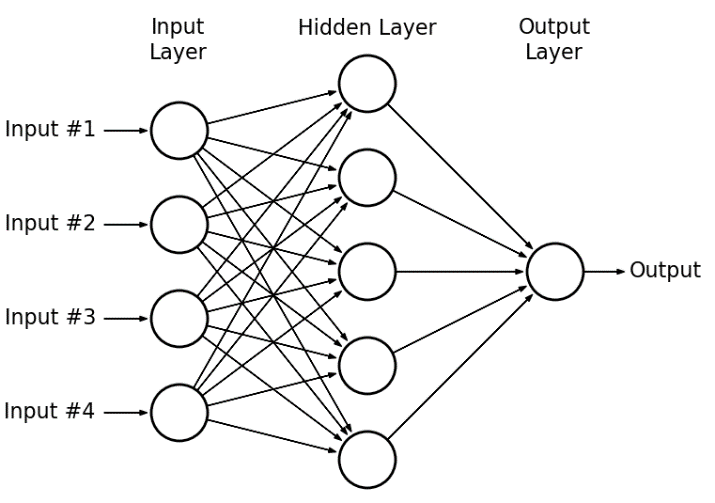
\includegraphics[width=0.45\textwidth]{mlp-schema.png}
\caption{Schemat sieci \textit{MLP} \cite{mlp-schema}. Ilość neuronów w warstwie wejściowej zazwyczaj odpowiada ilości parametrów wejściowych, a w warstwie wyjściowej ilości możliwych klas.}
\end{figure}


Wynik działania perceptronu wielowarstwowego możemy zapisać jako złożenie funkcji\cite{wiki}:
\begin{equation}
y = f^{(n)}(... f^{(3)}(f^{(2)}(f^{(1)}(x, \theta_1), \theta_2), \theta_3), \theta_n)
\end{equation}

gdzie:
\begin{description}
\item $y$ - wyjście sieci,
\item $x$ - wyjście sieci
\item $\theta$ - wagi.
\end{description}

W przeciwieństwie do perceptronu jednowarstwowego sieć ta może być wykorzystywana dla zbiorów, które nie są liniowo separowalne.


\pagebreak
\section{Zbiór danych}
W projekcie został wykorzystany zbiór danych \textit{Students Performance in Exams} \cite{kaggle-student} pochodzący z repozytorium \textit{Kaggle} \cite{kaggle}. Zawiera on 8 kolumn, zawierających informacje o studentach, takie jak:
\begin{itemize}
\item płeć,
\item rasa,
\item wykształcenie rodzica,
\item dieta dostarczana przez szkołę,
\item przystąpienie do kursu przygotowawczego,
\item wynik egzaminu SAT z części pisemnej,
\item wynik egzaminu SAT z części czytania,
\item wynik egzaminu SAT z części matematycznej.
\end{itemize}

W zbiorze wyróżnione zostały dwie płcie, pięć różnych ras, sześć poziomów wykształcenia rodzica ( uczęszczanie do szkoły średniej bez jej ukończenia, ukończenie szkoły średniej, uczęszczanie na uczelnię wyższą bez jej ukończenia, ukończenie \textit{community college}, ukończenie studiów licencjackich, ukończenie studiów magisterskich ). Dieta określona została przez dwie wartości: standardowa i pomniejszona, a przygotowania do egzaminu jako brak lub kurs ukończony. Wyniki egzaminów są liczbami całkowitymi z zakresu od 0 do 100.

Zbiór danych zawiera informacje dotyczące 1000 różnych studentów, dla wszystkich dane są kompletne. Jako zbiór uczący wybrane zostały kolumny 1-5, a wynikiem działania sieci będą rezultaty kolejnych egzaminów.

Statystyki dotyczące zbioru zostały przedstawione w rozdziale poniżej.

\subsection{Analiza zbioru danych}

\subsection{Korelacja pomiędzy danymi}
W ramach projektu został obliczony współczynnik korelacji \textit{Pearsona} pomiędzy danymi z repozytorium. Dzięki niemu możemy sprawdzić w jakim stopniu zależne są od siebie dane, a dzięki temu dostosować czynniki użyte do uczenia sieci.

Do obliczenia współczynnika korelacji została użyta funkcja pakietu MATLAB \verb\corr\.

\subsubsection {Korelacja pomiędzy wynikami egzaminów}
Na początku został wyznaczony współczynnik korelacji pomiędzy wynikami egzaminów. Jako ''Egzamin 1'' został przyjęty egzamin z części matematycznej, ''Egzamin 2'' - część z czytania, a ''Egzamin 3'' egzamin z części pisemnej. Otrzymane wyniki przedstawiono w tabeli poniżej.

\begin{table}[H]
\centering
\begin{tabular}{|c|c|c|} 
\hline
Egzamin 1 i 2 & Egzamin 1 i 3 & Egzamin 2 i 3  \\ 
\hline
0.6453 & 0.6435          &  0.8578 \\ 
\hline
\end{tabular}
\end{table}

Dla wszystkich kombinacji otrzymaliśmy wysokie wartości (większe od $0.6$), możemy więc uznać, że dane te są od siebie liniowo zależne. Największa korelacja występuje pomiędzy egzaminem 2 oraz 3, czyli egzaminem z czytania oraz z pisania - współczynnik jest równy $0.86$.

Na rysunkach poniżej zależności pomiędzy zbiorami zostały przedstawione w sposób graficzny.

\begin{figure}[H]
\centering
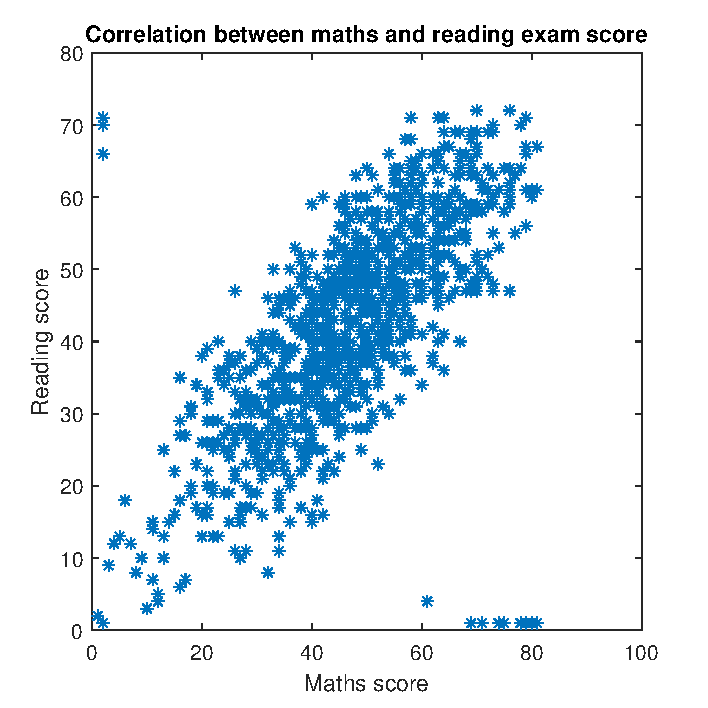
\includegraphics[width=0.45\textwidth]{korelacja_egzamin12.pdf}
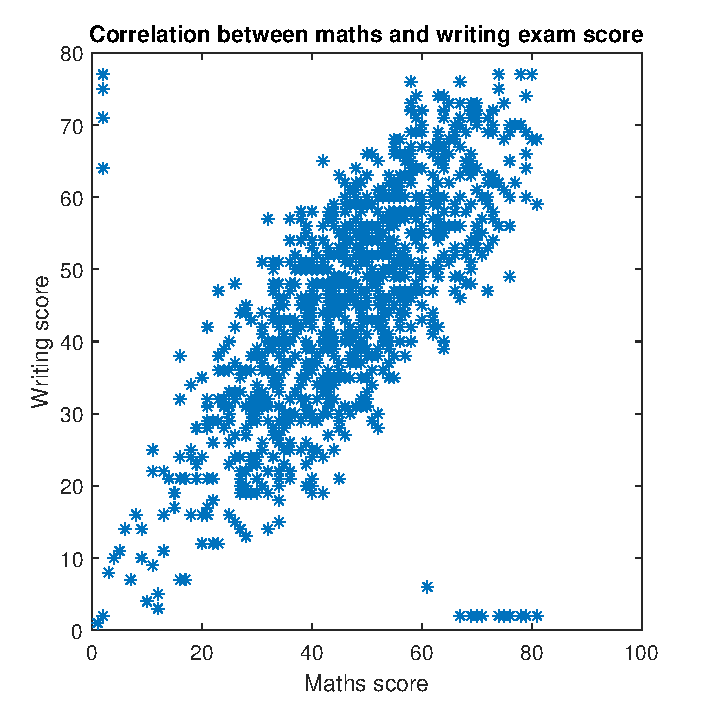
\includegraphics[width=0.45\textwidth]{korelacja_egzamin13.pdf}
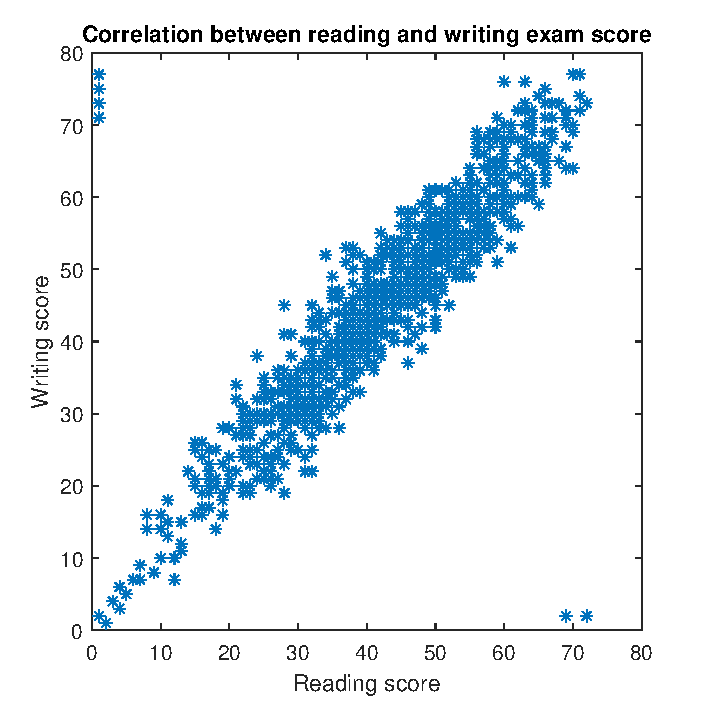
\includegraphics[width=0.45\textwidth]{korelacja_egzamin23.pdf}
\caption{Zależności pomiędzy wynikami egzaminów przedstawione w sposób graficzny.}
\end{figure}

\subsubsection {Korelacja pomiędzy czynnikami środowiskowymi a wynikami egzaminów}
W dalszej części analizy zbioru danych została zbadana zależność pomiędzy czynnikami, będącymi wejściem sieci neuronowej, a wynikami kolejnych egzaminów. Otrzymane współczynniki korelacji przedstawiono w tabeli poniżej.

\begin{table}[H]
\centering
\begin{tabular}{|c|c|c|c|} 
\hline
 Czynnik środowiskowy & Egzamin 1 & Egzamin 2 & Egzamin 3  \\ 
\hline
Płeć & 0.1558  &  -0.1886 &  -0.2396  \\ 
\hline
Rasa &  0.1771  &  0.0770   & 0.0907 \\ 
\hline
Wykształcenie rodzica &  -0.0584  & -0.0306 &  -0.0571  \\ 
\hline
Przystąpienie do kursu & 0.3269  &  0.1906  &  0.2182  \\ 
\hline
Dieta &  -0.1564  & -0.1838   & -0.2647  \\ 
\hline
\end{tabular}
\end{table}

Otrzymane wartości są dość niskie, nie istnieje wyraźna korelacja pomiędzy którąś z tych cech, a wynikami. Najmniejszą zależność obserwujemy pomiędzy wynikami, wykształceniem rodziców - są one najbliższe zeru. Największe znaczenie ma przystąpienie do kursu przygotowawczego, w dalszej kolejności dieta oraz płeć.

\begin{figure}[H]
\centering
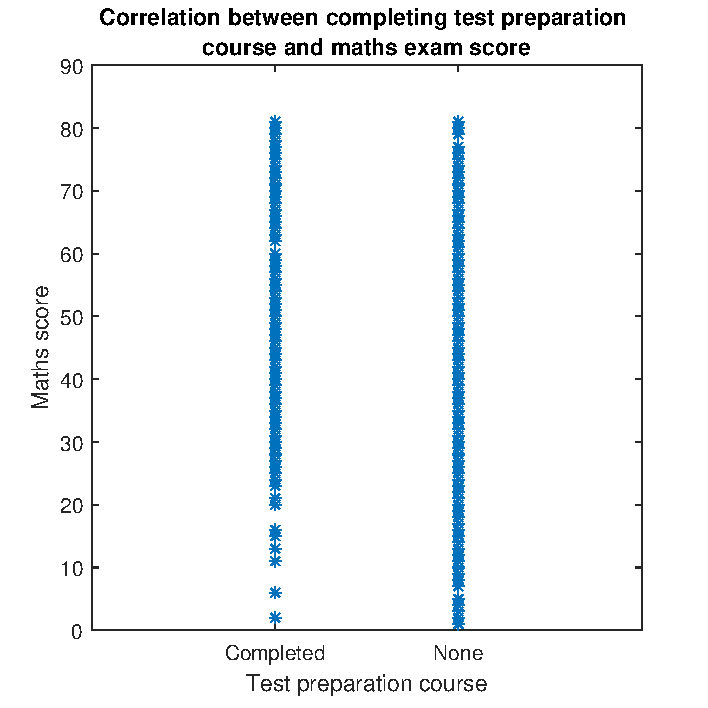
\includegraphics[width=0.45\textwidth]{korelacja_kurs_egzamin_1.pdf}
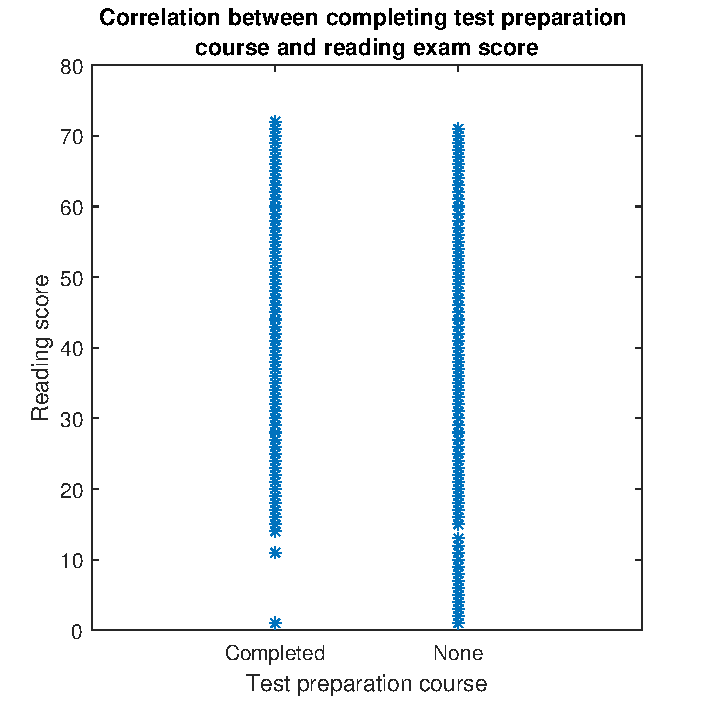
\includegraphics[width=0.45\textwidth]{korelacja_kurs_egzamin_2.pdf}
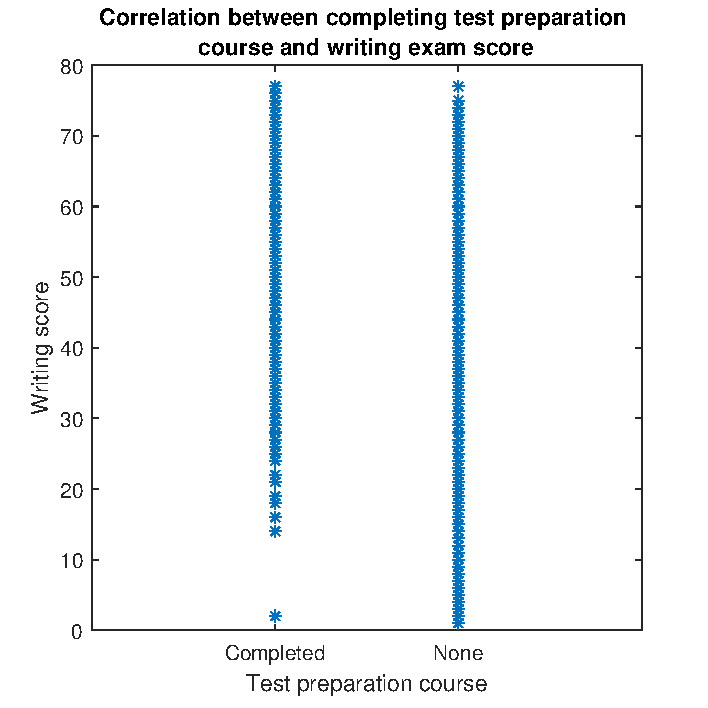
\includegraphics[width=0.45\textwidth]{korelacja_kurs_egzamin_3.pdf}
\caption{Zależności pomiędzy wynikami egzaminów a ukończeniem kursu przygotowawczego przedstawiona w sposób graficzny. Na rysunkach można zauważyć, że osoby które ukończyły kurs, uzyskiwały wynik większy niż 15, ale osoby, które nie ukończyły kursu uzyskiwały równie wysokie wyniki, co osoby po kursie. Wyjątek stanowi egzamin z części matematycznej - tu osób, które uzyskały wysoki wynik bez ukończenia kursu jest mniej. }
\end{figure}

\pagebreak
\section{Poszukiwanie najlepszej konfiguracji sieci neuronowej}
% że regresja, co testowaliśmy i dlaczego takie
% mlp 
Przeprowadzono badanie błędu średniokwadratowego dla uczenia oraz testu różnych konfiguracji funkcji aktywacji, ilości warstw ukrytych oraz ilości neuronów w poszczególnych warstwach.
Przetestowano konfigurację sieci o jednej oraz dwóch warstwach, z wykorzystaniem różnych kombinacji funkcji:
\begin{enumerate}
\item \verb+logsig+
\item \verb+tansig+
\item \verb+purelin+
\item \verb+radbas+
\end{enumerate}
Dla każdej konfiguracji zbadano również wpływ ilości neuronów w poszczególnych warstwach. Ilość neuronów zmieniano między  10 a 100 ze skokiem 10. Wykresy błędów dla wybranych konfiguracji znajdują się na następnych stronach.

\subsection{Wykresy pudełkowe}
Otrzymane błędy uczenia oraz testu dla różnych konfiguracji przedstawiono przy pomocy tak zwanych wykresów pudełkowych z wąsami. Przykład takiego wykresu pokazano na rysunku \ref{fig:exampleBoxplot}.


Na wykresie zielone diamenty symbolizują wartości średnie z N prób, czerwona linia wewnątrz oznacza medianę. Górna granica pudełka to trzeci kwartyl ($Q_3$), natomiast dolna to kwaryl pierwszy ($Q_1$). Dolny i górny ''wąs'' reprezentują kolejno wartości $Q_1 - 1.5 IQR$ oraz  $Q_3 +  1.5 IQR$, gdzie $IQR$ to rozstęp ćwiartkowy, obliczany jako $IQR = Q_3 - Q_1$. Czerwonymi plusami zaznaczono wartości odstające.


\begin{figure}[H]
\centering
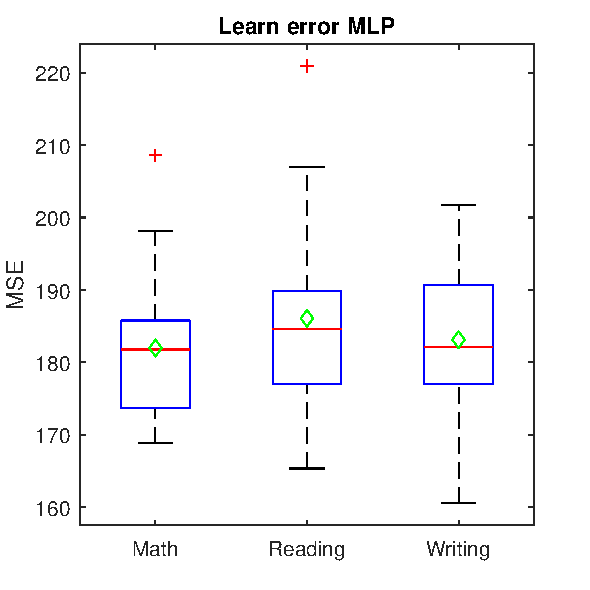
\includegraphics[width=0.45\textwidth]{tansig_purelin_20_learnBoxplot.pdf}
\caption{Przykład wykresu pudełkowego pokazującego błędy dla różnych egzaminów.} \label{fig:exampleBoxplot}
\end{figure}

\subsection{Otrzymane błędy uczenia i testu dla różnych konfiguracji}

\begin{figure}[H]
\centering
\begin{subfigure}[t]{0.48\textwidth} 
\centering
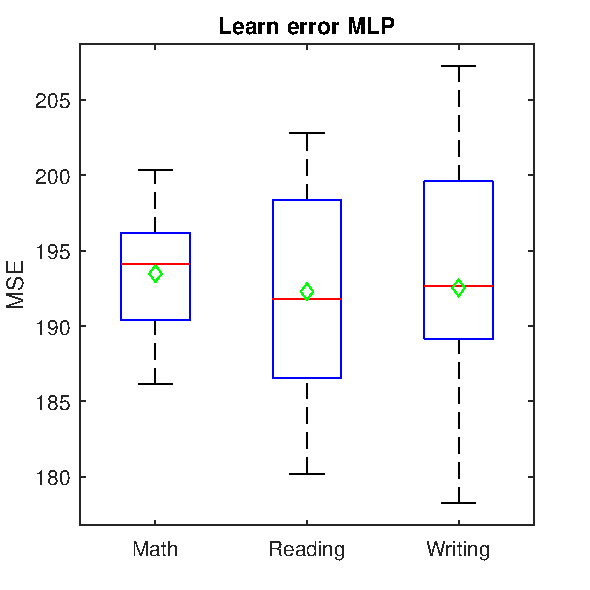
\includegraphics[height=2.2in]{purelin_purelin_20_learnBoxplot.pdf}
\caption{MSE uczenia dla 20 neuronów.}
\end{subfigure}
~~
\begin{subfigure}[t]{0.48\textwidth} 
\centering
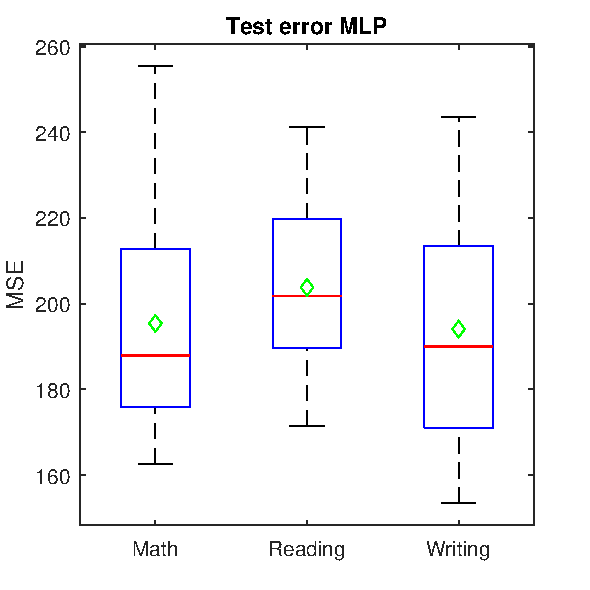
\includegraphics[height=2.2in]{purelin_purelin_20_testBoxplot.pdf}
\caption{MSE testu dla 20 neuronów.}
\end{subfigure}

\begin{subfigure}[t]{0.48\textwidth} 
\centering
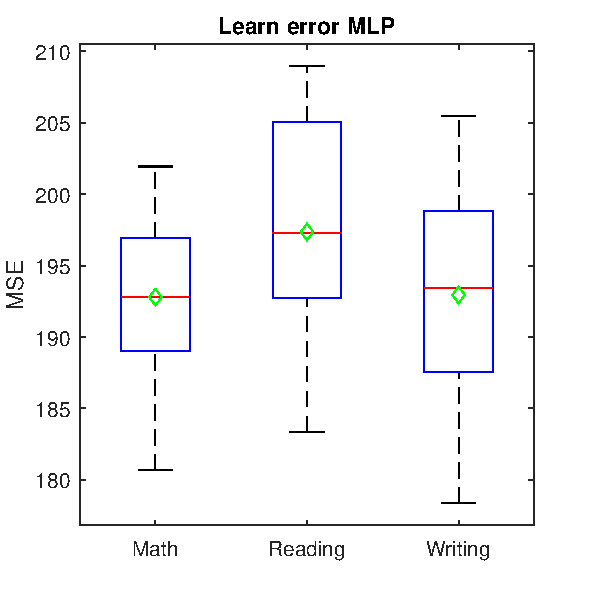
\includegraphics[height=2.2in]{purelin_purelin_50_learnBoxplot.pdf}
\caption{MSE uczenia dla 50 neuronów.}
\end{subfigure}
~~
\begin{subfigure}[t]{0.48\textwidth} 
\centering
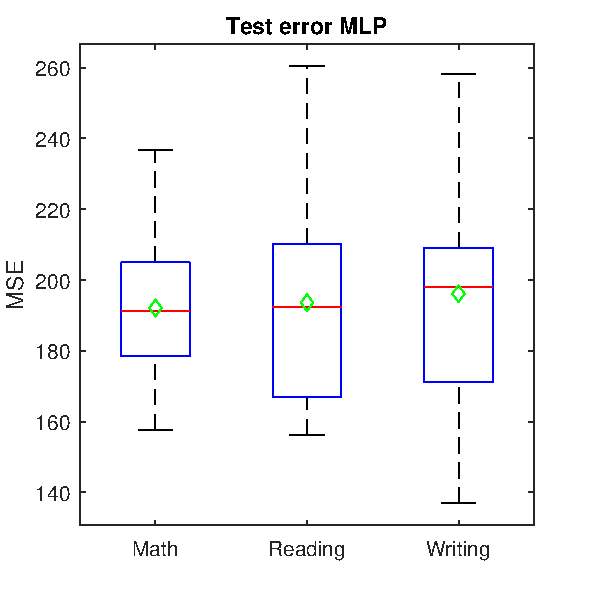
\includegraphics[height=2.2in]{purelin_purelin_50_testBoxplot.pdf}
\caption{MSE testu dla 50 neuronów.}
\end{subfigure}
\caption{Błąd uczenia i testowania sieci dla X prób dla kolejnych egzaminów, \textbf{funkcje: purelin, purelin}.}
\end{figure}

Pierwszym omawianym zestawieniem jest prosty przykład dla kombinacji funkcji purelin oraz purelin. Otrzymane wartości błędów były jednymi z najmniejszych wśród wszystkich konfiguracji, z akceptowalnym odchyleniem. W przypadku tak prostej sieci ilość neuronów nie wpłynęła praktycznie wcale na otrzymane wyniki.

\begin{figure}[H]
\centering
\begin{subfigure}[t]{0.48\textwidth} 
\centering
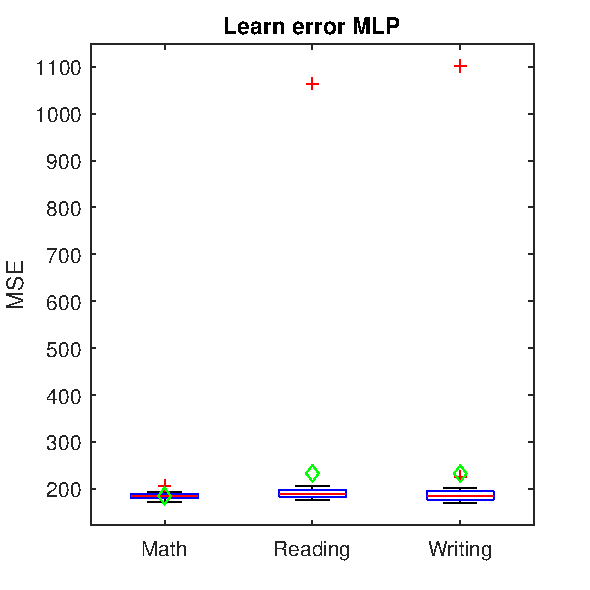
\includegraphics[height=2.2in]{tansig_tansig_20_learnBoxplot.pdf}
\caption{MSE uczenia dla 20 neuronów.}
\end{subfigure}
~~
\begin{subfigure}[t]{0.48\textwidth} 
\centering
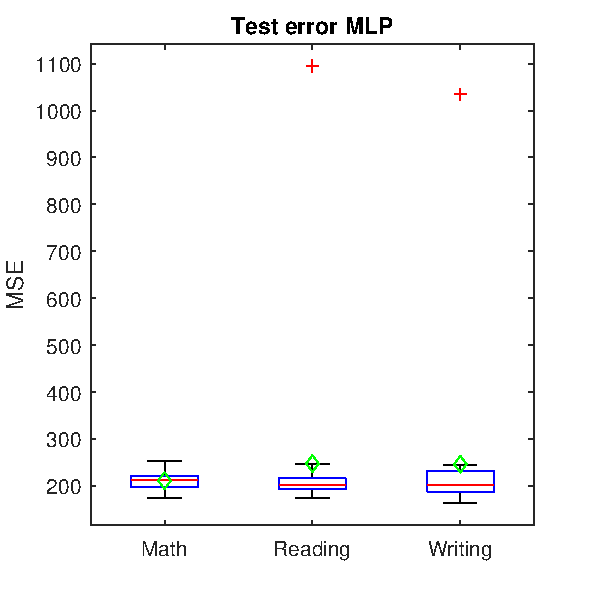
\includegraphics[height=2.2in]{tansig_tansig_20_testBoxplot.pdf}
\caption{MSE testu dla 20 neuronów.}
\end{subfigure}

\begin{subfigure}[t]{0.48\textwidth} 
\centering
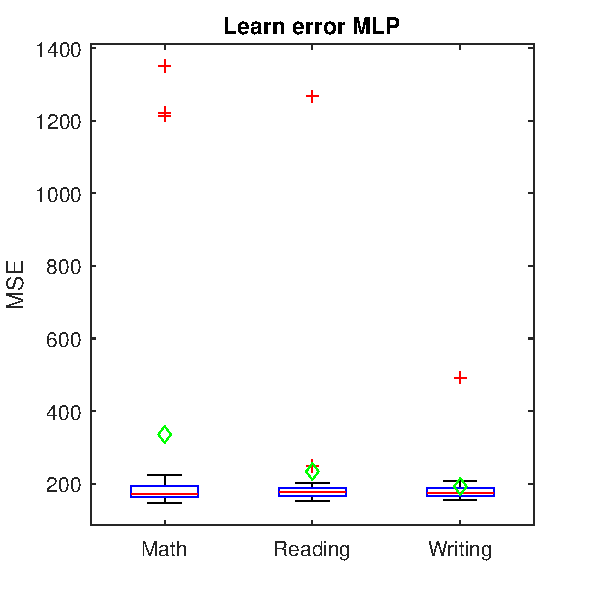
\includegraphics[height=2.2in]{tansig_tansig_50_learnBoxplot.pdf}
\caption{MSE uczenia dla 50 neuronów.}
\end{subfigure}
~~
\begin{subfigure}[t]{0.48\textwidth} 
\centering
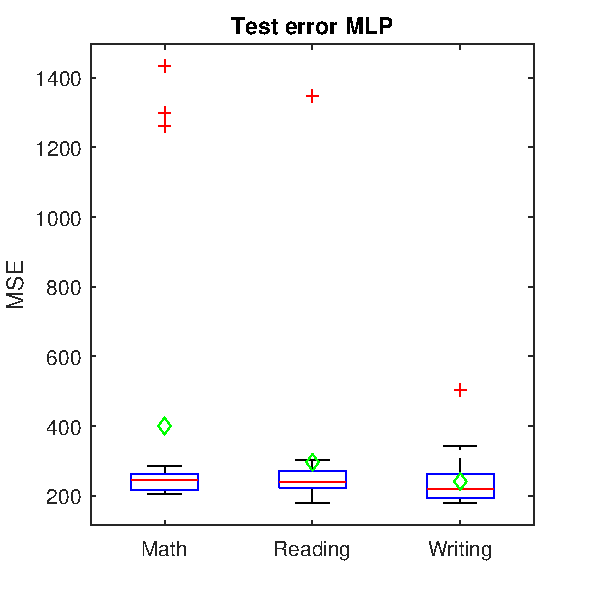
\includegraphics[height=2.2in]{tansig_tansig_50_testBoxplot.pdf}
\caption{MSE testu dla 50 neuronów.}
\end{subfigure}

\caption{Błąd uczenia i testowania sieci dla X prób dla kolejnych egzaminów, \textbf{funkcje: tansig, tansig}.}
\end{figure}
Przykładem jednej z konfiguracji, która daje mierne rezultaty jest konfiguracja z wykorzystaniem funkcji tansig oraz tansig na wyjściu. Wartości błędów były jednymi z większych, jednak istotny jest fakt, że wyniki dla trzeciego egzaminu były zbieżne, w przeciwieństwie do większości pozostałych konfiguracji. Ilość neuronów nie miała dużego wpływu na otrzymywane błędy.



\begin{figure}[H]
\centering
\begin{subfigure}[t]{0.48\textwidth} 
\centering
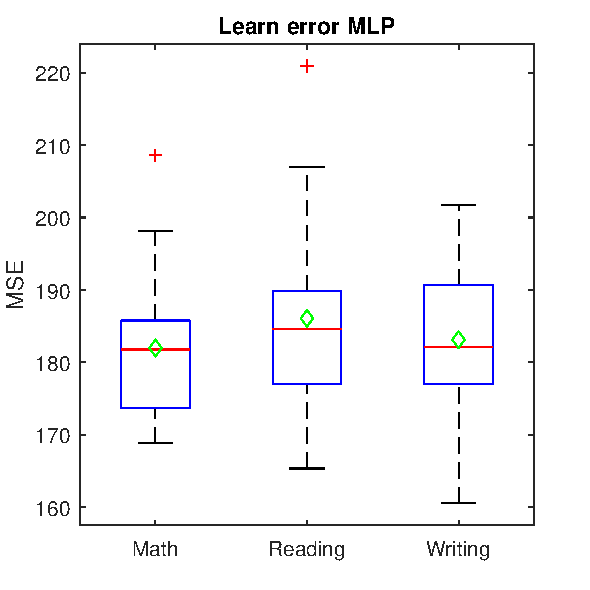
\includegraphics[height=2.2in]{tansig_purelin_20_learnBoxplot.pdf}
\caption{MSE uczenia dla 20 neuronów.}
\end{subfigure}
~~
\begin{subfigure}[t]{0.48\textwidth} 
\centering
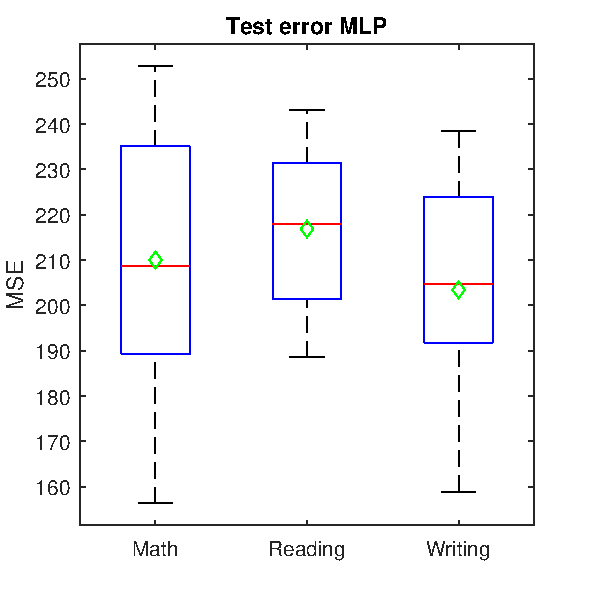
\includegraphics[height=2.2in]{tansig_purelin_20_testBoxplot.pdf}
\caption{MSE testu dla 20 neuronów.}
\end{subfigure}

\begin{subfigure}[t]{0.48\textwidth} 
\centering
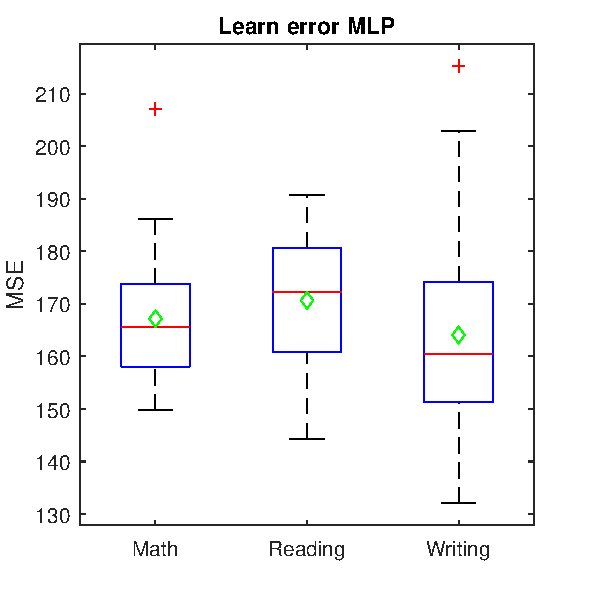
\includegraphics[height=2.2in]{tansig_purelin_50_learnBoxplot.pdf}
\caption{MSE uczenia dla 50 neuronów.}
\end{subfigure}
~~
\begin{subfigure}[t]{0.48\textwidth} 
\centering
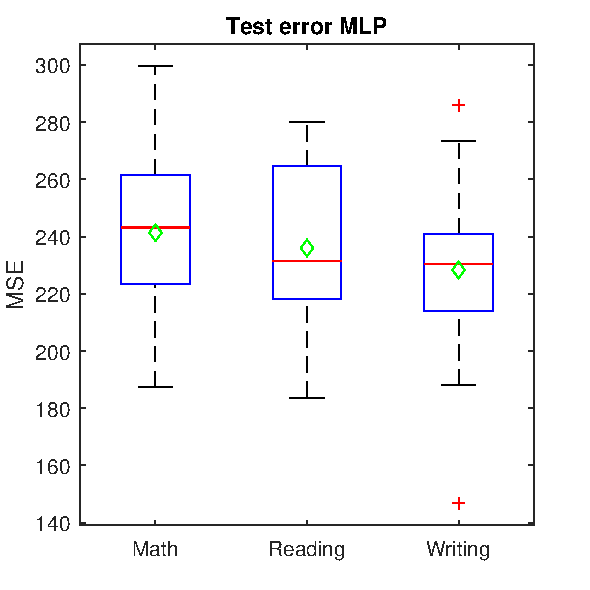
\includegraphics[height=2.2in]{tansig_purelin_50_testBoxplot.pdf}
\caption{MSE testu dla 50 neuronów.}
\end{subfigure}

\caption{Błąd uczenia i testowania sieci dla X prób dla kolejnych egzaminów, \textbf{funkcje: tansig, purelin}.}
\end{figure}


Kombinacja tansig oraz purelin daje bardzo niskie wartości błędu w porównaniu z pozostałymi metodami, jednak z dość dużym rozstrzałem między otrzymywanymi wartościami. Błedy uczenia nieznacznie spadały wraz ze wzrostem ilości neuronów w warstwie, jednak tendencja dla testu była odwrotna. Najlepsze wyniki udało się uzyskać dla 20 oraz 30 neuronów.




\begin{figure}[H]
\centering
\begin{subfigure}[t]{0.48\textwidth} 
\centering
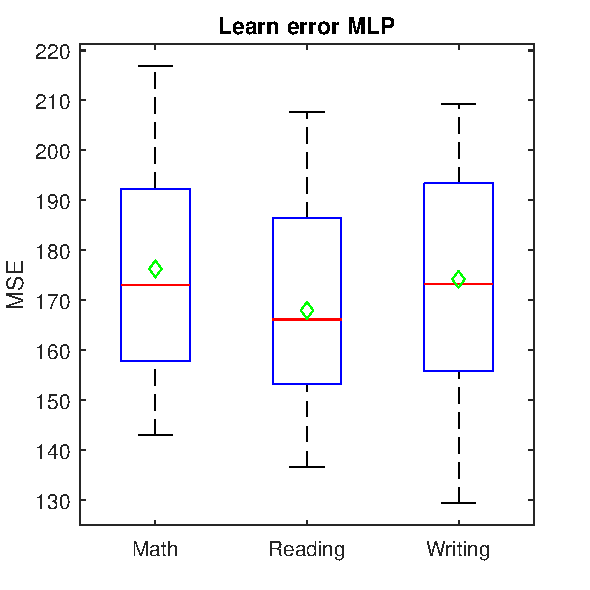
\includegraphics[height=2.2in]{radbas_tansig_purelin_20_learnBoxplot.pdf}
\caption{MSE uczenia dla  40 neuronów w pierwszej warstwie, 20 w drugiej.}
\end{subfigure}
~~
\begin{subfigure}[t]{0.48\textwidth} 
\centering
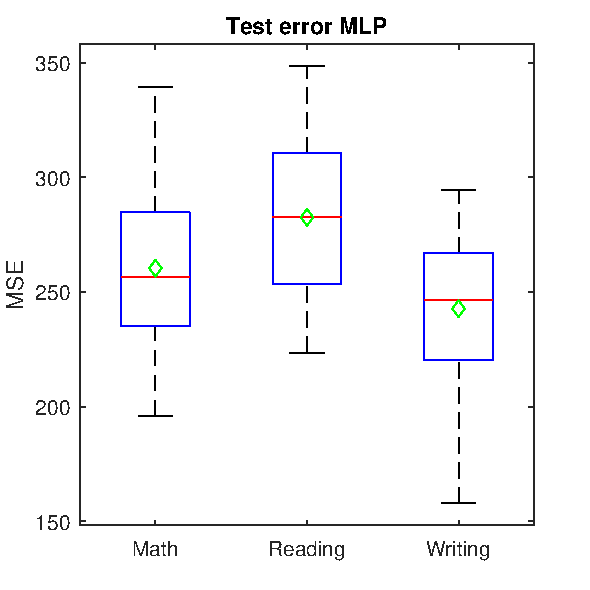
\includegraphics[height=2.2in]{radbas_tansig_purelin_20_testBoxplot.pdf}
\caption{MSE testu dla  40 neuronów w pierwszej warstwie, 20 w drugiej.}
\end{subfigure}

\begin{subfigure}[t]{0.48\textwidth} 
\centering
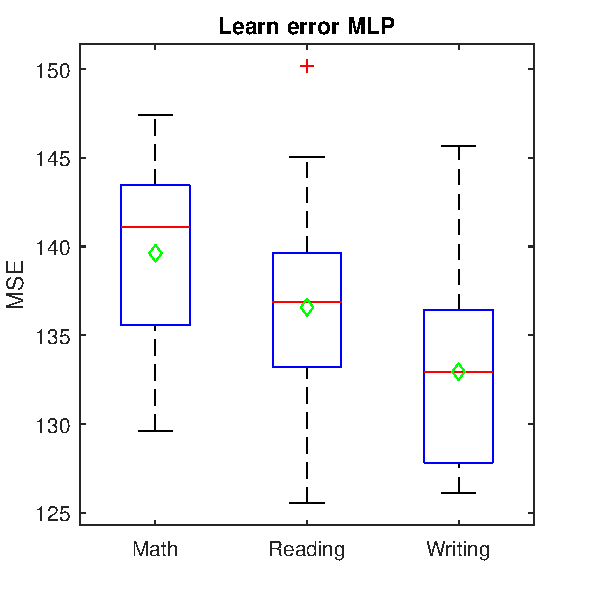
\includegraphics[height=2.2in]{radbas_tansig_purelin_50_learnBoxplot.pdf}
\caption{MSE uczenia dla  100 neuronów w pierwszej warstwie, 50 w drugiej.}
\end{subfigure}
~~
\begin{subfigure}[t]{0.48\textwidth} 
\centering
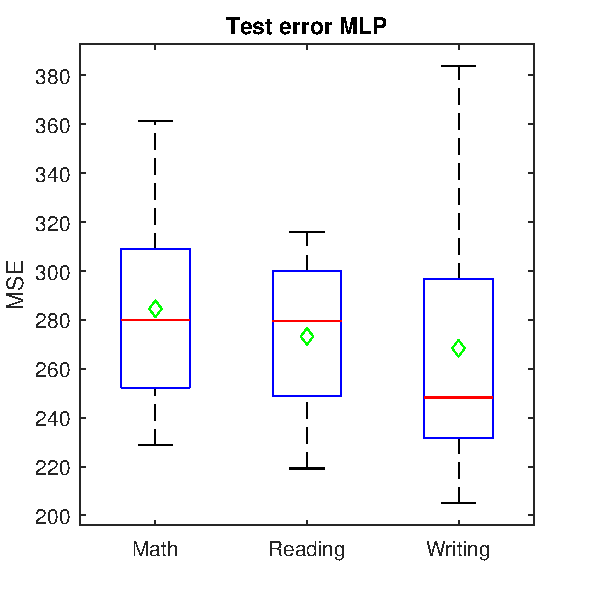
\includegraphics[height=2.2in]{radbas_tansig_purelin_50_testBoxplot.pdf}
\caption{MSE testu dla 100 neuronów w pierwszej warstwie, 50 w drugiej.}
\end{subfigure}

\caption{Błąd uczenia i testowania sieci dla X prób dla kolejnych egzaminów, \textbf{funkcje: radbas, tansig, purelin}.}
\end{figure}

Postanowiono również przetestować sieci o dwóch warstwach w bardziej egzotycznych konfiguracjach, dla przykładu konfiguracja radbas, tansig, purelin dała zadziwiająco niskie wartości błędów dla próby uczenia, który gwałtownie zmieniał się wraz z dokładaniem ilości neuronów. Pod względem błędu uczenia była to najlepsza konfiguracja.




\begin{figure}[H]
\centering
\begin{subfigure}[t]{0.48\textwidth} 
\centering
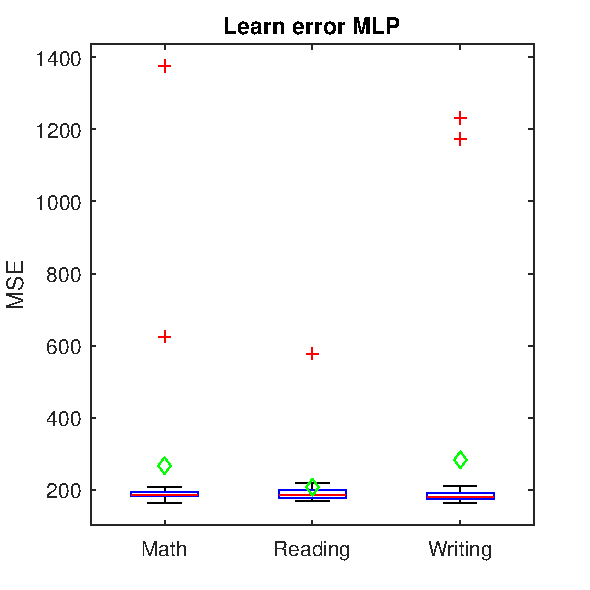
\includegraphics[height=2.2in]{logsig_tansig_tansig_20_learnBoxplot.pdf}
\caption{MSE uczenia dla  50 neuronów w pierwszej warstwie, 50 w drugiej.}
\end{subfigure}
~~
\begin{subfigure}[t]{0.48\textwidth} 
\centering
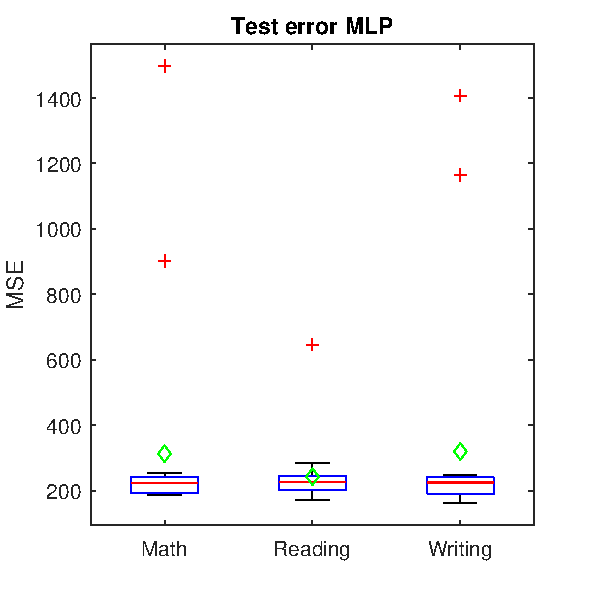
\includegraphics[height=2.2in]{logsig_tansig_tansig_20_testBoxplot.pdf}
\caption{MSE testu dla  50 neuronów w pierwszej warstwie, 50 w drugiej.}
\end{subfigure}

\begin{subfigure}[t]{0.48\textwidth} 
\centering
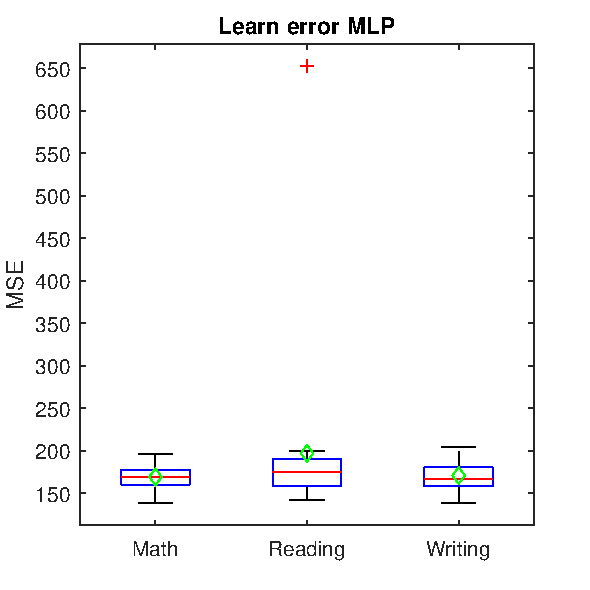
\includegraphics[height=2.2in]{logsig_tansig_tansig_50_learnBoxplot.pdf}
\caption{MSE uczenia dla  50 neuronów w pierwszej warstwie, 50 w drugiej.}
\end{subfigure}
~~
\begin{subfigure}[t]{0.48\textwidth} 
\centering
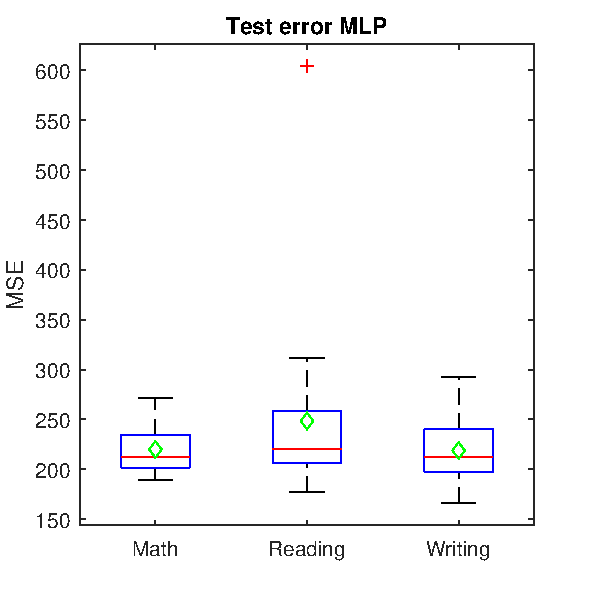
\includegraphics[height=2.2in]{logsig_tansig_tansig_50_testBoxplot.pdf}
\caption{MSE testu dla 50 neuronów w pierwszej warstwie, 50 w drugiej.}
\end{subfigure}

\caption{Błąd uczenia i testowania sieci dla X prób dla kolejnych egzaminów, \textbf{funkcje: logisg, tansig, tansig}.}
\end{figure}

Kombinacja logsig, tansig oraz tansig dała ciekawe rezultaty, wartości błędu dla wszystkich prób nie licząc trzeciego egzaminu były do siebie zbliżone. Wyniki dla trzeciego egzaminu jednak zbyt odstają od reszty, by móc brać tą konfiguracje w kolejnych badaniach.

W zestawieniu nie objęto wykresów dla pozostałych kombinacji (na przykład tansig, tansig),  gdyż niezależnie od ilości neuronów wyniki były bardzo złe.

\vspace{0.5cm}

Poniżej przedstawione zostały przykładowe wyniki dla najlepszej (purelin, purelin, 20 neuronów) i najgorszej sieci (tansig, tansig, 50 neuronów w warstwie ukrytej), dla zbioru testującego.

\begin{figure}[H]
\begin{subfigure}[t]{0.48\textwidth} 
\centering
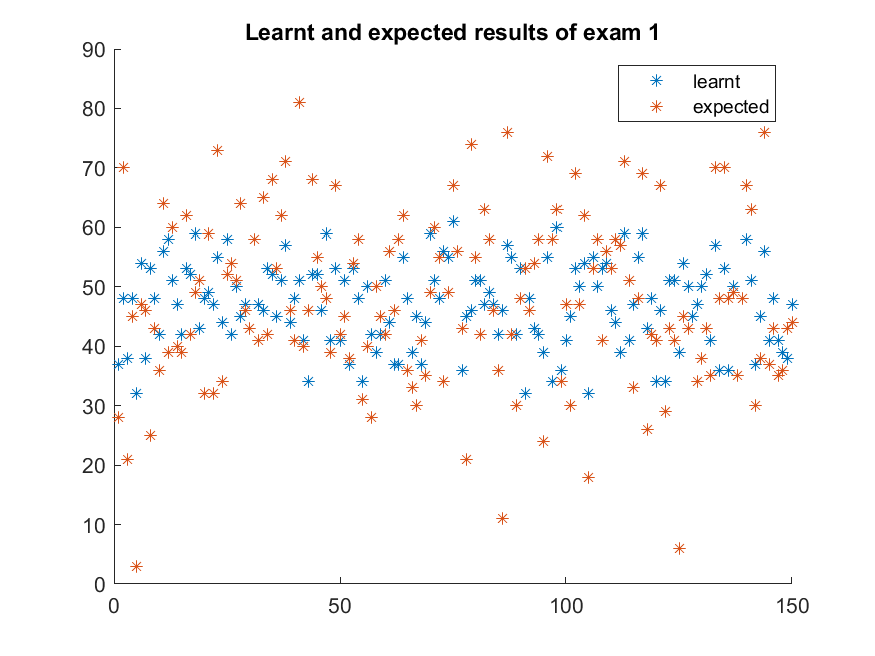
\includegraphics[height=2.2in]{best_results_1.png}
\caption{Oczekiwane i znalezione wyniki dla najlepszej sieci dla egzaminu 1 (matematyka).}
\end{subfigure}
~~
\begin{subfigure}[t]{0.48\textwidth} 
\centering
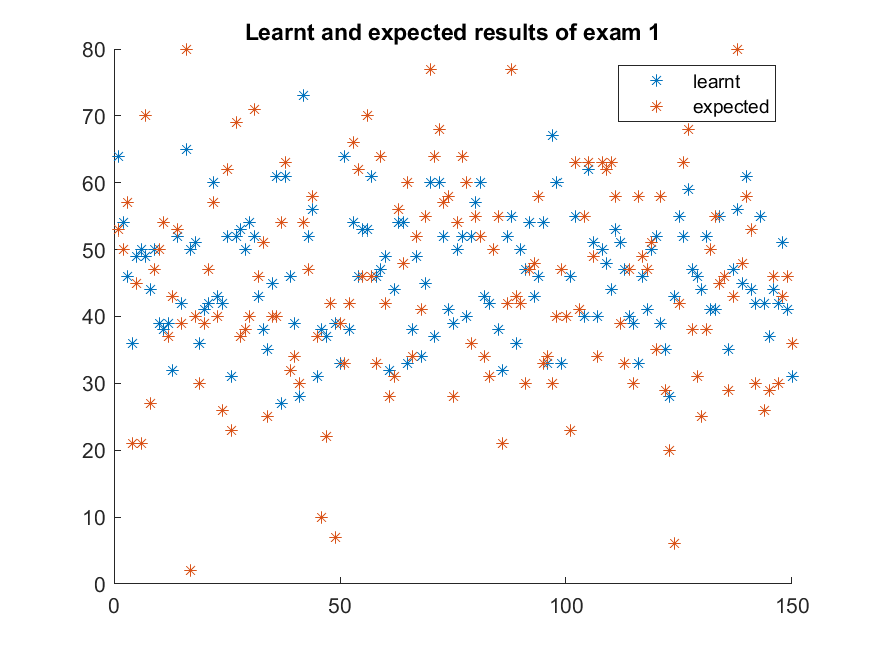
\includegraphics[height=2.2in]{worst_exam_1.png}
\caption{Oczekiwane i znalezione wyniki dla najgorszej sieci dla egzaminu 1 (matematyka).}
\end{subfigure}

\begin{subfigure}[t]{0.48\textwidth} 
\centering
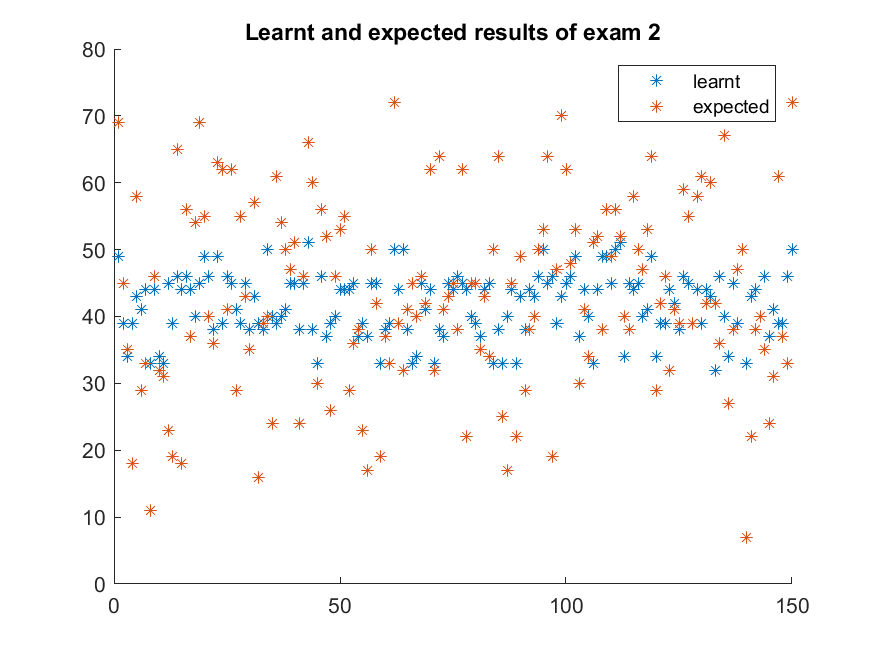
\includegraphics[height=2.2in]{best_results_2.png}
\caption{Oczekiwane i znalezione wyniki dla najlepszej sieci dla egzaminu 2 (czytanie).}
\end{subfigure}
~~
\begin{subfigure}[t]{0.48\textwidth} 
\centering
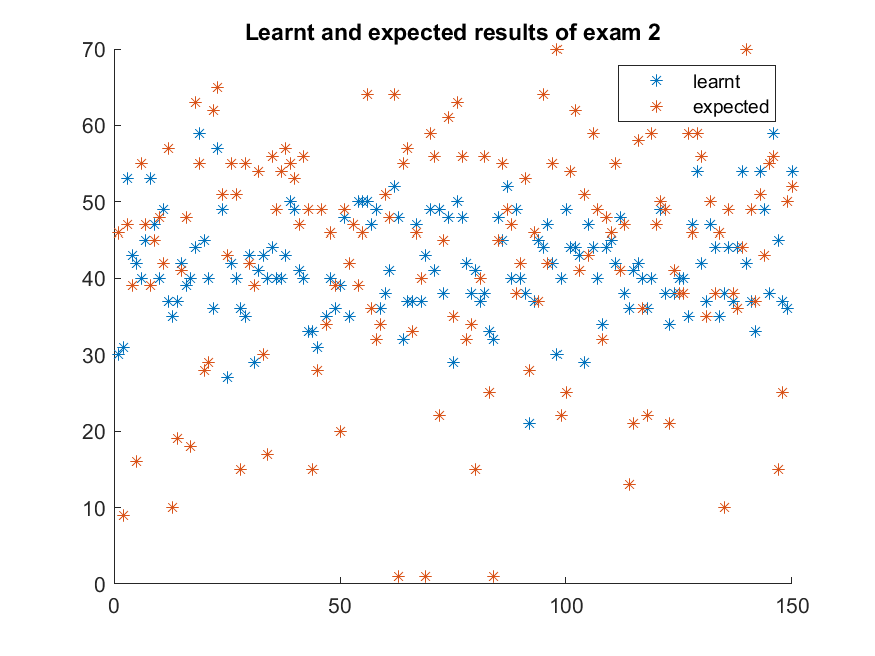
\includegraphics[height=2.2in]{worst_exam_2.png}
\caption{Oczekiwane i znalezione wyniki dla najgorszej sieci dla egzaminu 2 (czytanie).}
\end{subfigure}

\begin{subfigure}[t]{0.48\textwidth} 
\centering
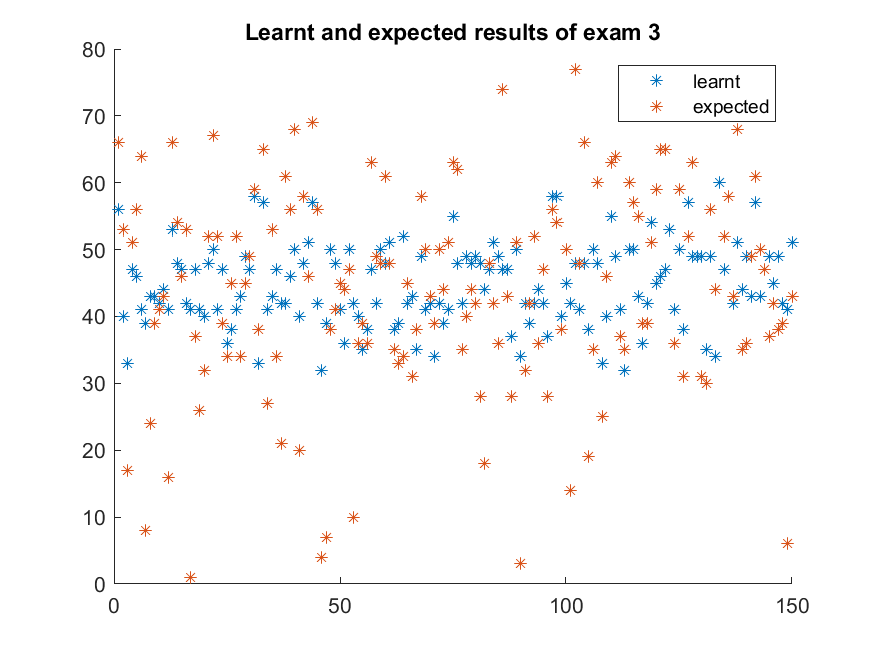
\includegraphics[height=2.2in]{best_results_3.png}
\caption{Oczekiwane i znalezione wyniki dla najlepszej sieci dla egzaminu 3 (pisanie).}
\end{subfigure}
~~
\begin{subfigure}[t]{0.48\textwidth} 
\centering
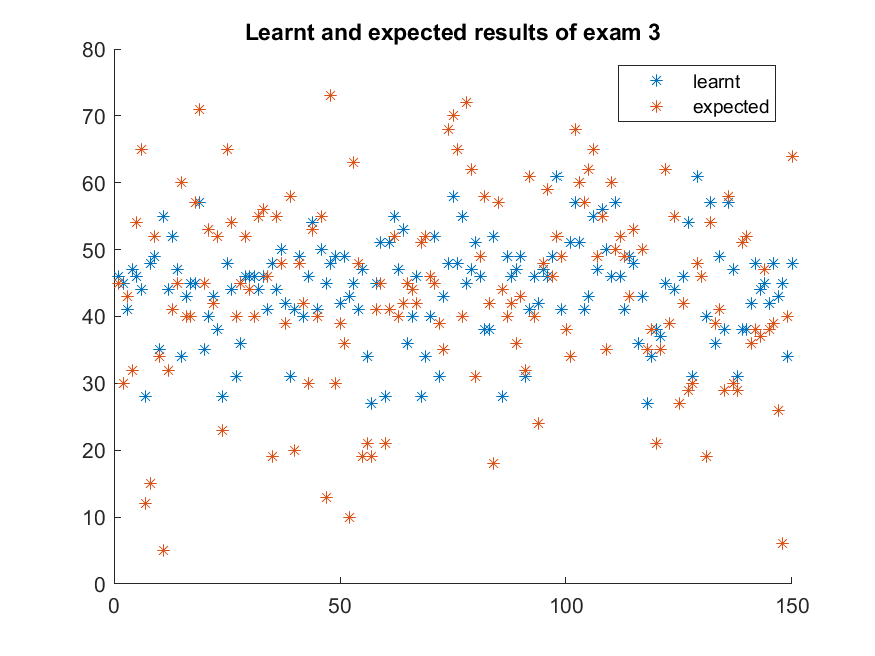
\includegraphics[height=2.2in]{worst_exam_3.png}
\caption{Oczekiwane i znalezione wyniki dla najgorszej sieci dla egzaminu 3 (pisanie).}
\end{subfigure}
\end{figure}

Powyższe wyniki pochodzą z pojedynczego uruchomienia programu, przy każdym uczeniu wynik działania będzie trochę inny. 

Na rysunkach możemy zauważyć, że dla najlepszej sieci wyniki pochodzące z sieci są bardziej skupione w okolicy średniej liczby punktów. W przypadku najgorszej sieci otrzymane dane są bardziej ''rozproszone'' -  nieliniowy kształt odpowiedzi niekorzystnie wypływa na wyniki sieci.

\pagebreak
\section{Badanie wpływu ilości kolumn na jakość sieci}

Dla wybranych najlepszych parametrów sieci zostało przeprowadzone uczenie ze zmniejszoną ilością kolumn. Celem tego zabiegu było zbadanie, jaki wpływ mają te czynniki na jakość działania sieci. 

\subsection{Uzyskane błędy w przypadku usunięcia pierwszej kolumny}
Ze zbioru uczącego została usunięta kolumna informująca o \textbf{płci} studenta. Wyniki działania takiej sieci przedstawiono poniżej.

\begin{figure}[H]
\centering
\begin{subfigure}[t]{0.48\textwidth} 
\centering
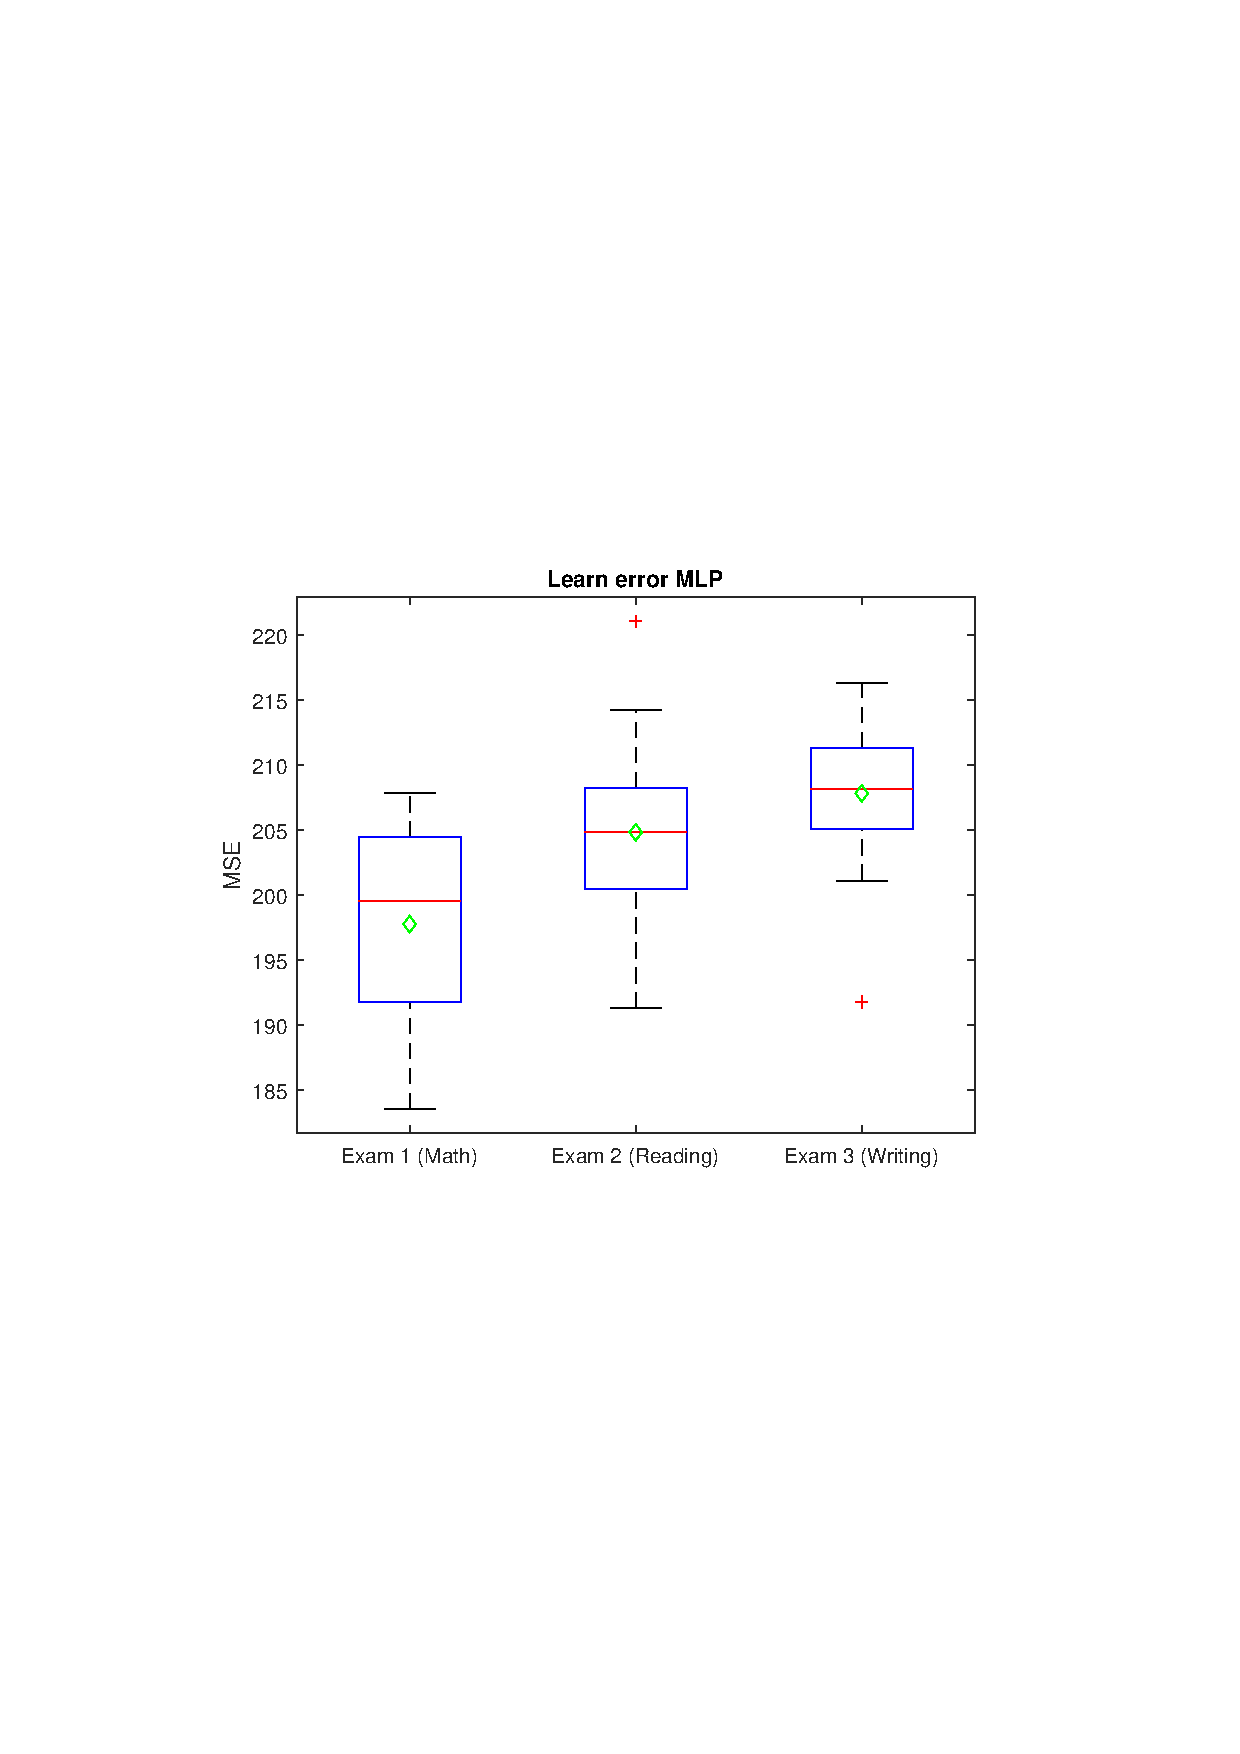
\includegraphics[height=3.3in]{purelin_purelin_20_without_1_learnBoxplot.pdf}
\caption{MSE uczenia dla  20 neuronów w pierwszej warstwie.}
\end{subfigure}
~~
\begin{subfigure}[t]{0.48\textwidth} 
\centering
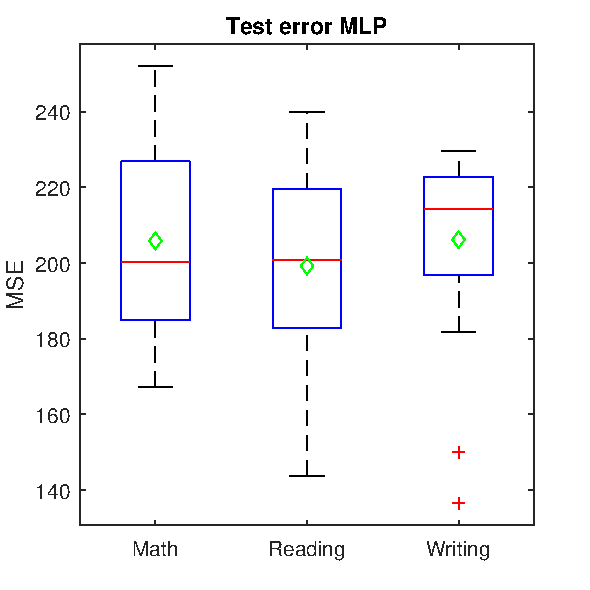
\includegraphics[height=3.3in]{purelin_purelin_20_without_1_testBoxplot.pdf}
\caption{MSE testu dla  20  neuronów w pierwszej warstwiej.}
\end{subfigure}

\caption{Błąd uczenia i testowania sieci w przypadku usunięcia pierwszej kolumny z danymi, \textbf{funkcje: purelin, purelin}.}
\end{figure}

\subsection{Uzyskane błędy w przypadku usunięcia drugiej  kolumny}
Poniżej przedstawione zostały błędy uczenia oraz testowania sieci przy usunięciu kolumny informującej o \textbf{rasie} studenta.

\begin{figure}[H]
\centering
\begin{subfigure}[t]{0.48\textwidth} 
\centering
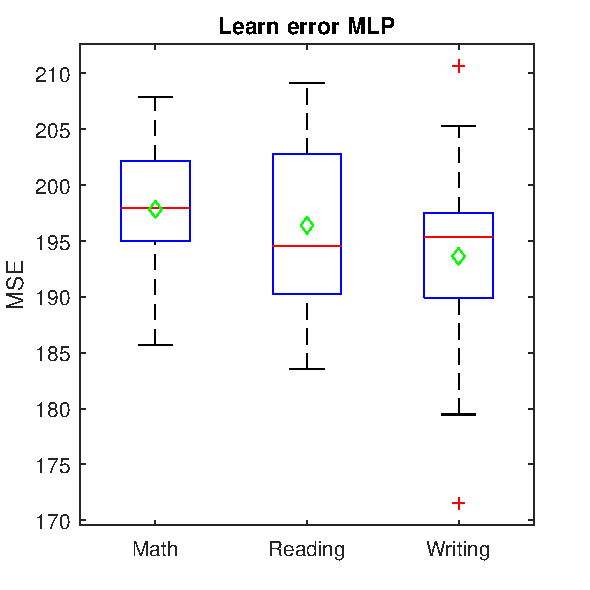
\includegraphics[height=3.3in]{purelin_purelin_20_without_2_learnBoxplot.pdf}
\caption{MSE uczenia dla  20 neuronów w pierwszej warstwie.}
\end{subfigure}
~~
\begin{subfigure}[t]{0.48\textwidth} 
\centering
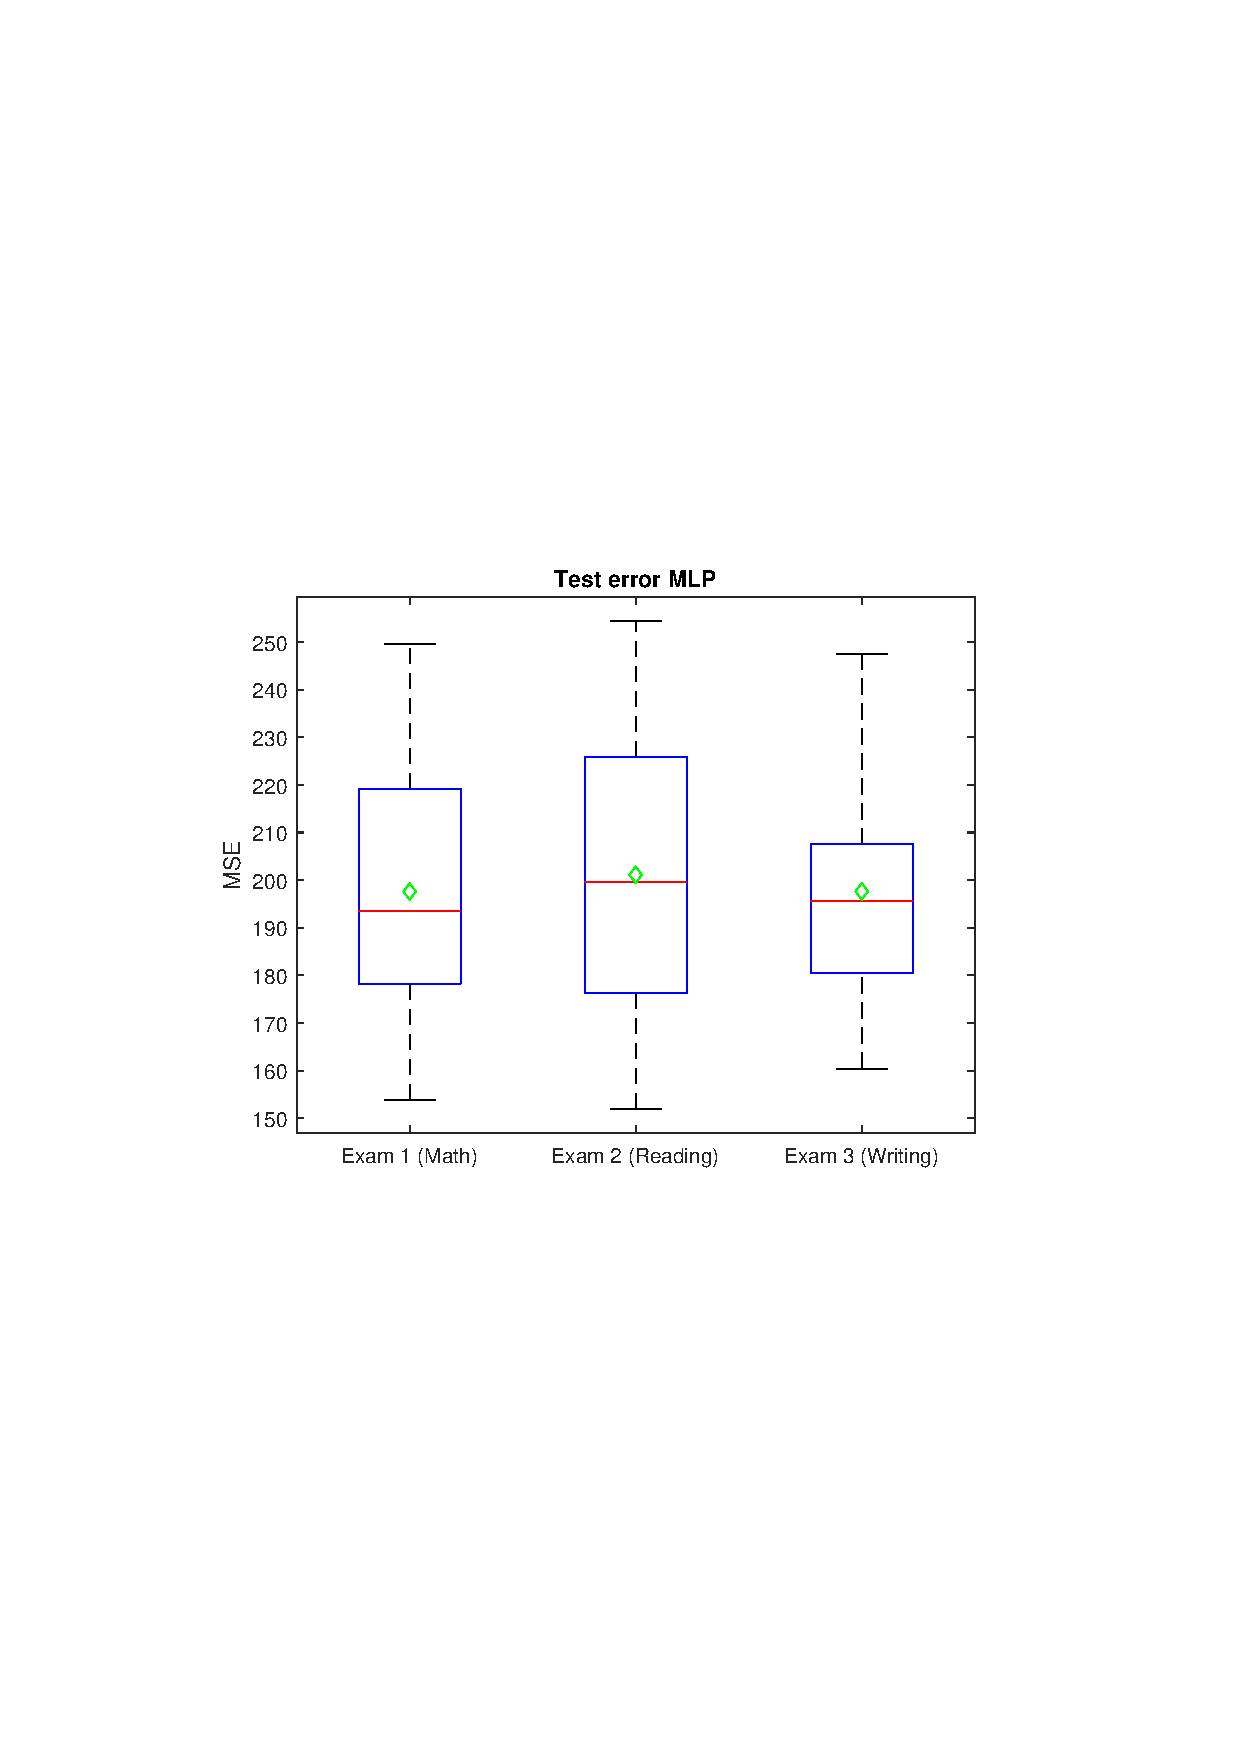
\includegraphics[height=3.3in]{purelin_purelin_20_without_2_testBoxplot.pdf}
\caption{MSE testu dla  20  neuronów w pierwszej warstwiej.}
\end{subfigure}

\caption{Błąd uczenia i testowania sieci w przypadku usunięcia drugiej kolumny z danymi, \textbf{funkcje: purelin, purelin}.}
\end{figure}


\subsection{Uzyskane błędy w przypadku usunięcia trzeciej kolumny}
Ze zbioru uczącego usunięta została kolumna informująca o wykształceniu rodzica.

\begin{figure}[H]
\centering
\begin{subfigure}[t]{0.48\textwidth} 
\centering
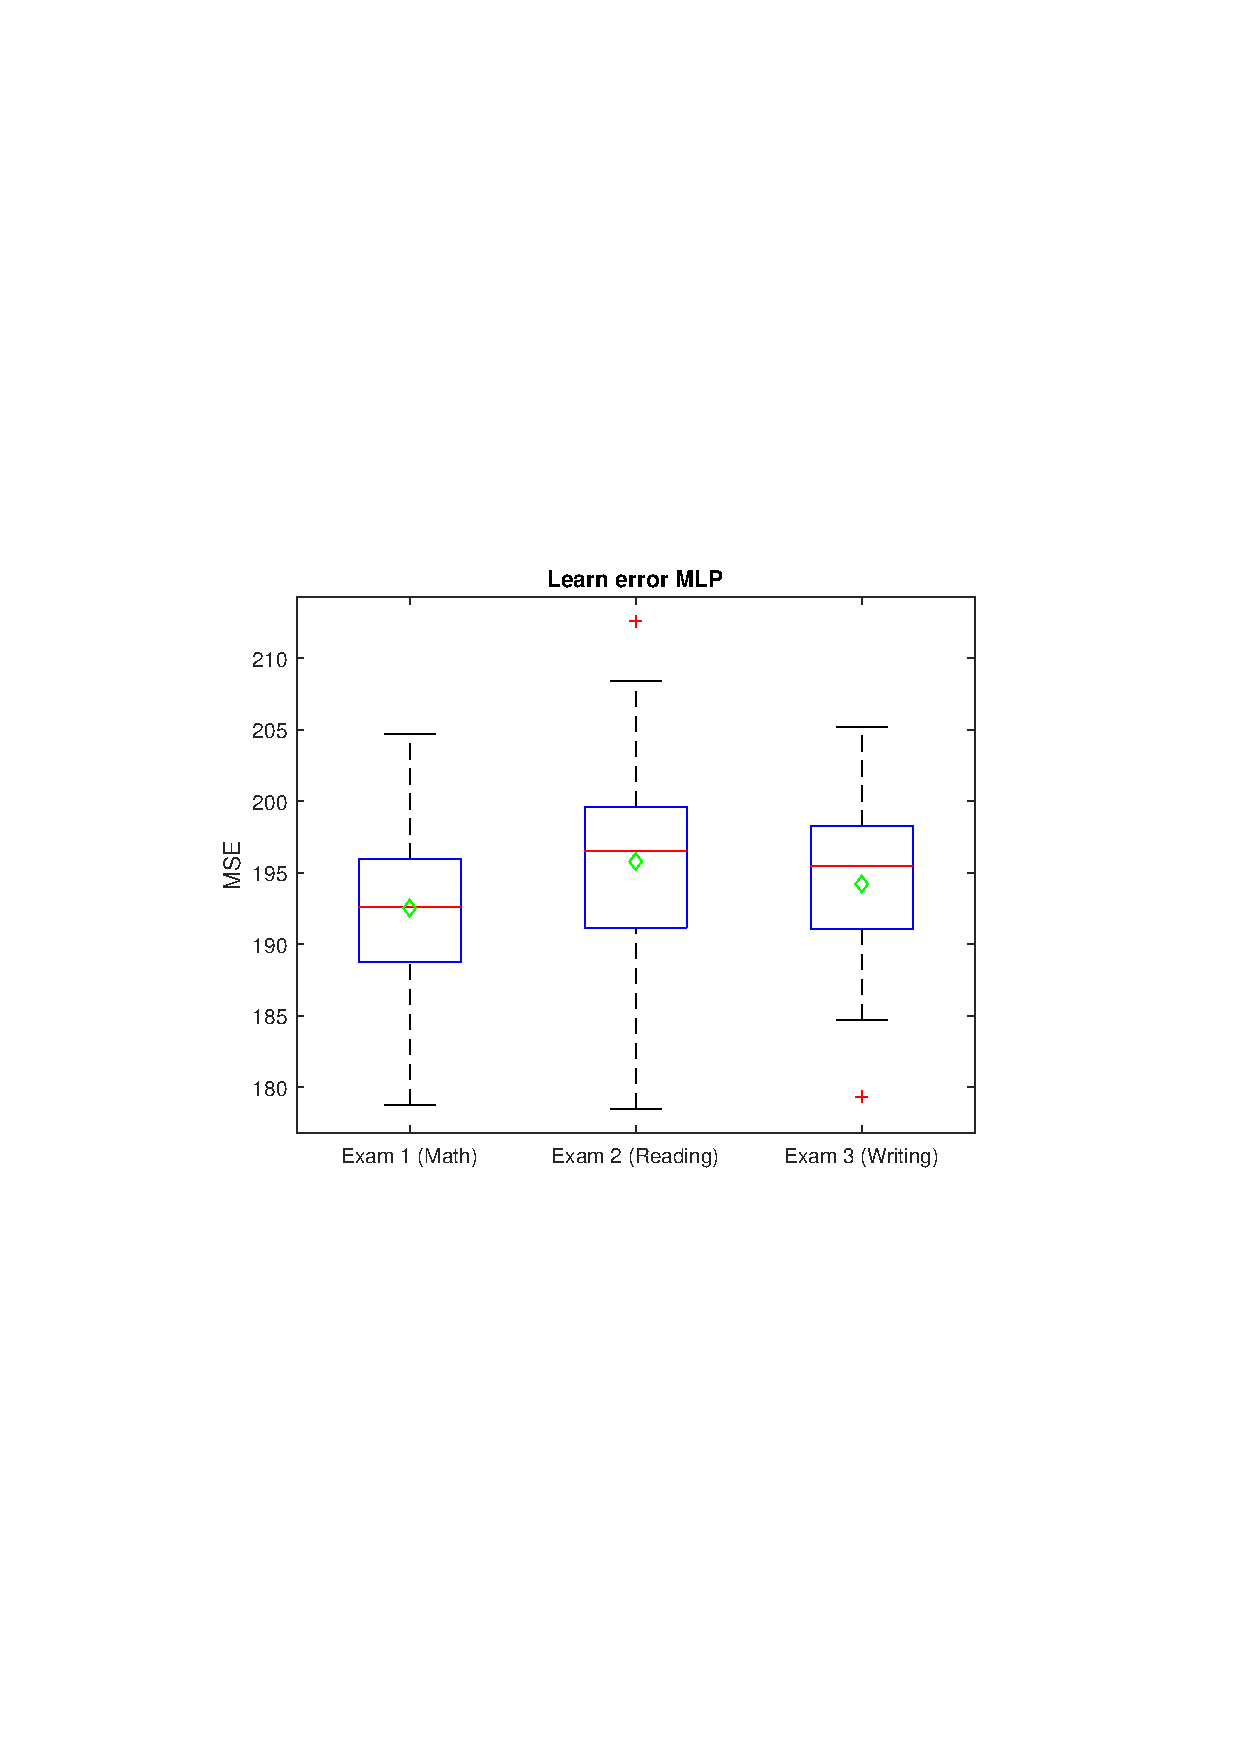
\includegraphics[height=3.3in]{purelin_purelin_20_without_3_learnBoxplot.pdf}
\caption{MSE uczenia dla  20 neuronów w pierwszej warstwie.}
\end{subfigure}
~~
\begin{subfigure}[t]{0.48\textwidth} 
\centering
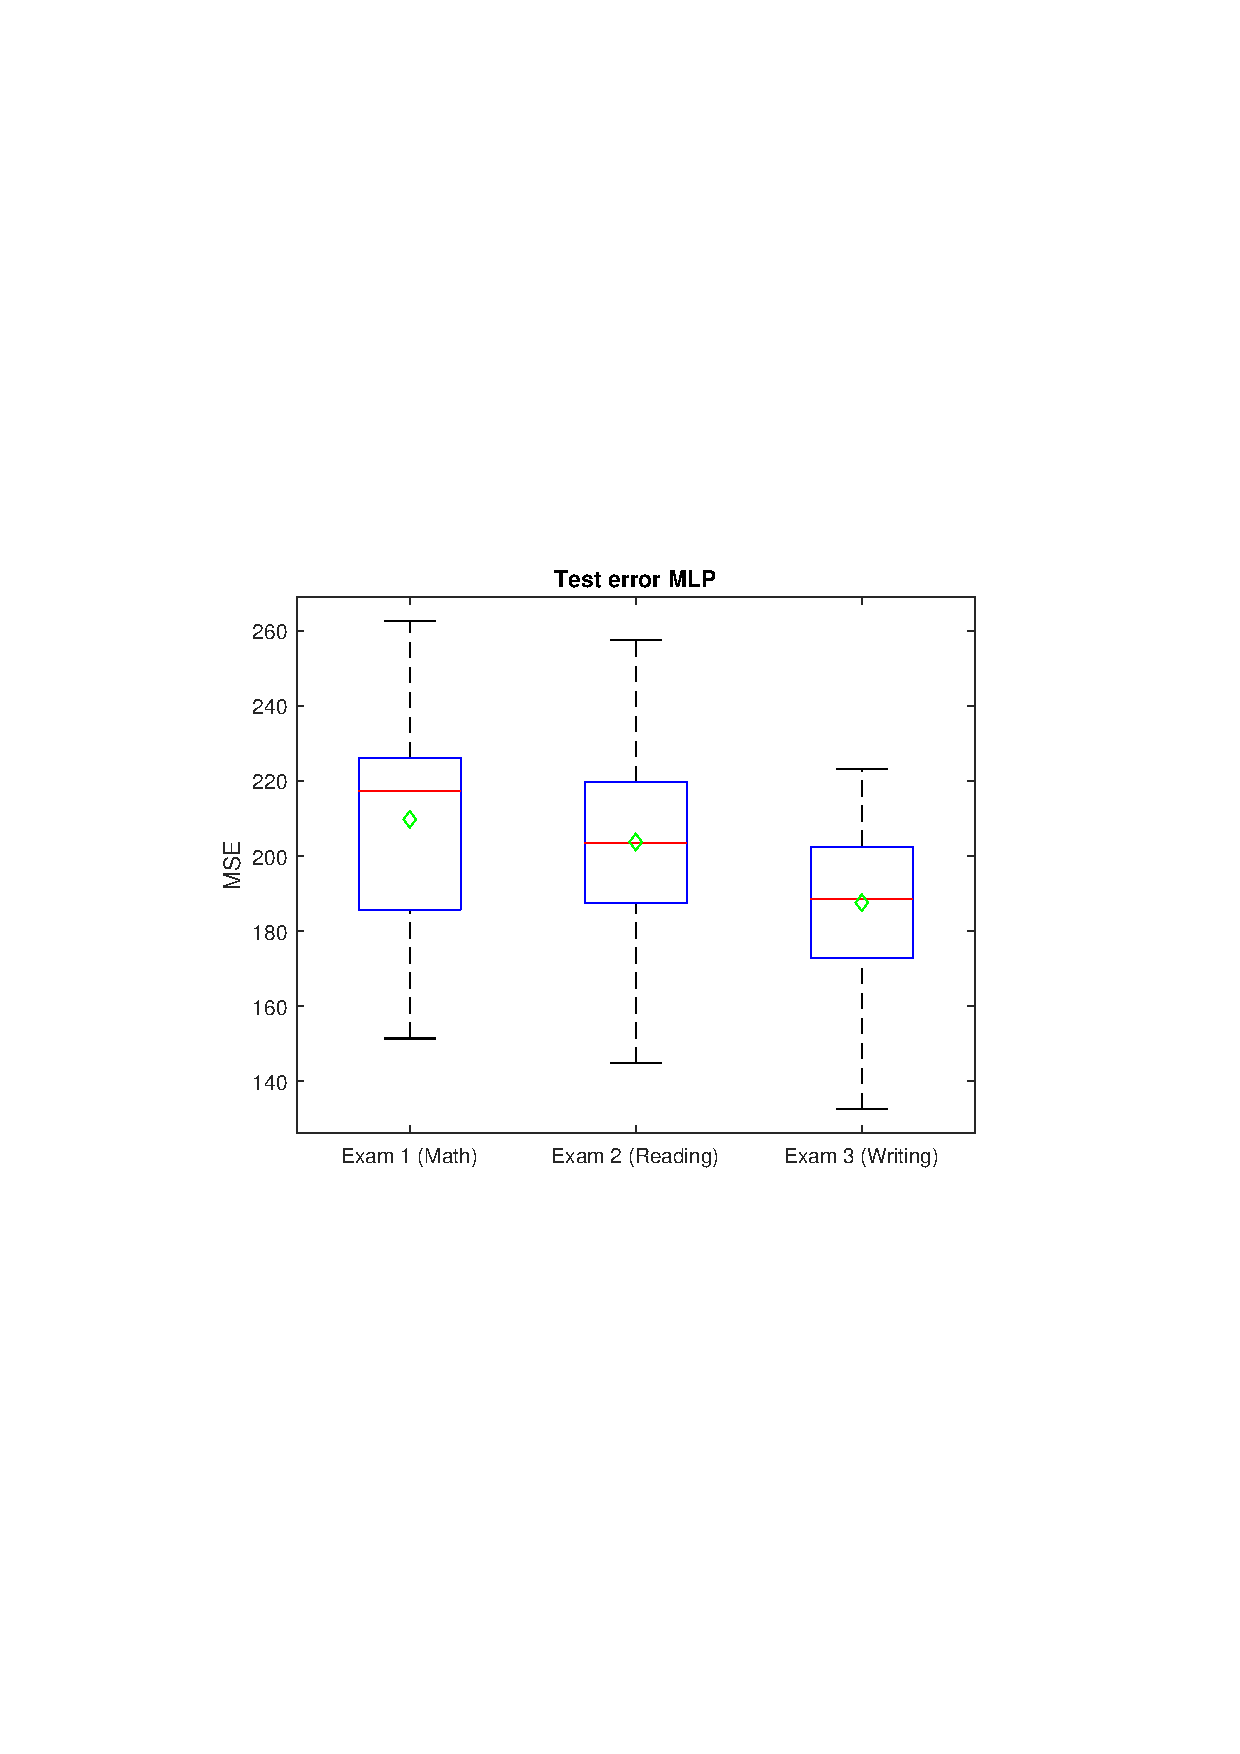
\includegraphics[height=3.3in]{purelin_purelin_20_without_3_testBoxplot.pdf}
\caption{MSE testu dla  20  neuronów w pierwszej warstwiej.}
\end{subfigure}

\caption{Błąd uczenia i testowania sieci w przypadku usunięcia trzeciej  kolumny z danymi, \textbf{funkcje: purelin, purelin}.}
\end{figure}

\subsection{Uzyskane błędy w przypadku usunięcia czwartej kolumny}
Poniżej przedstawiono błędy sieci w przypadku usunięcia czwartej kolumny, informującej o diecie studenta.
\begin{figure}[H]
\centering
\begin{subfigure}[t]{0.48\textwidth} 
\centering
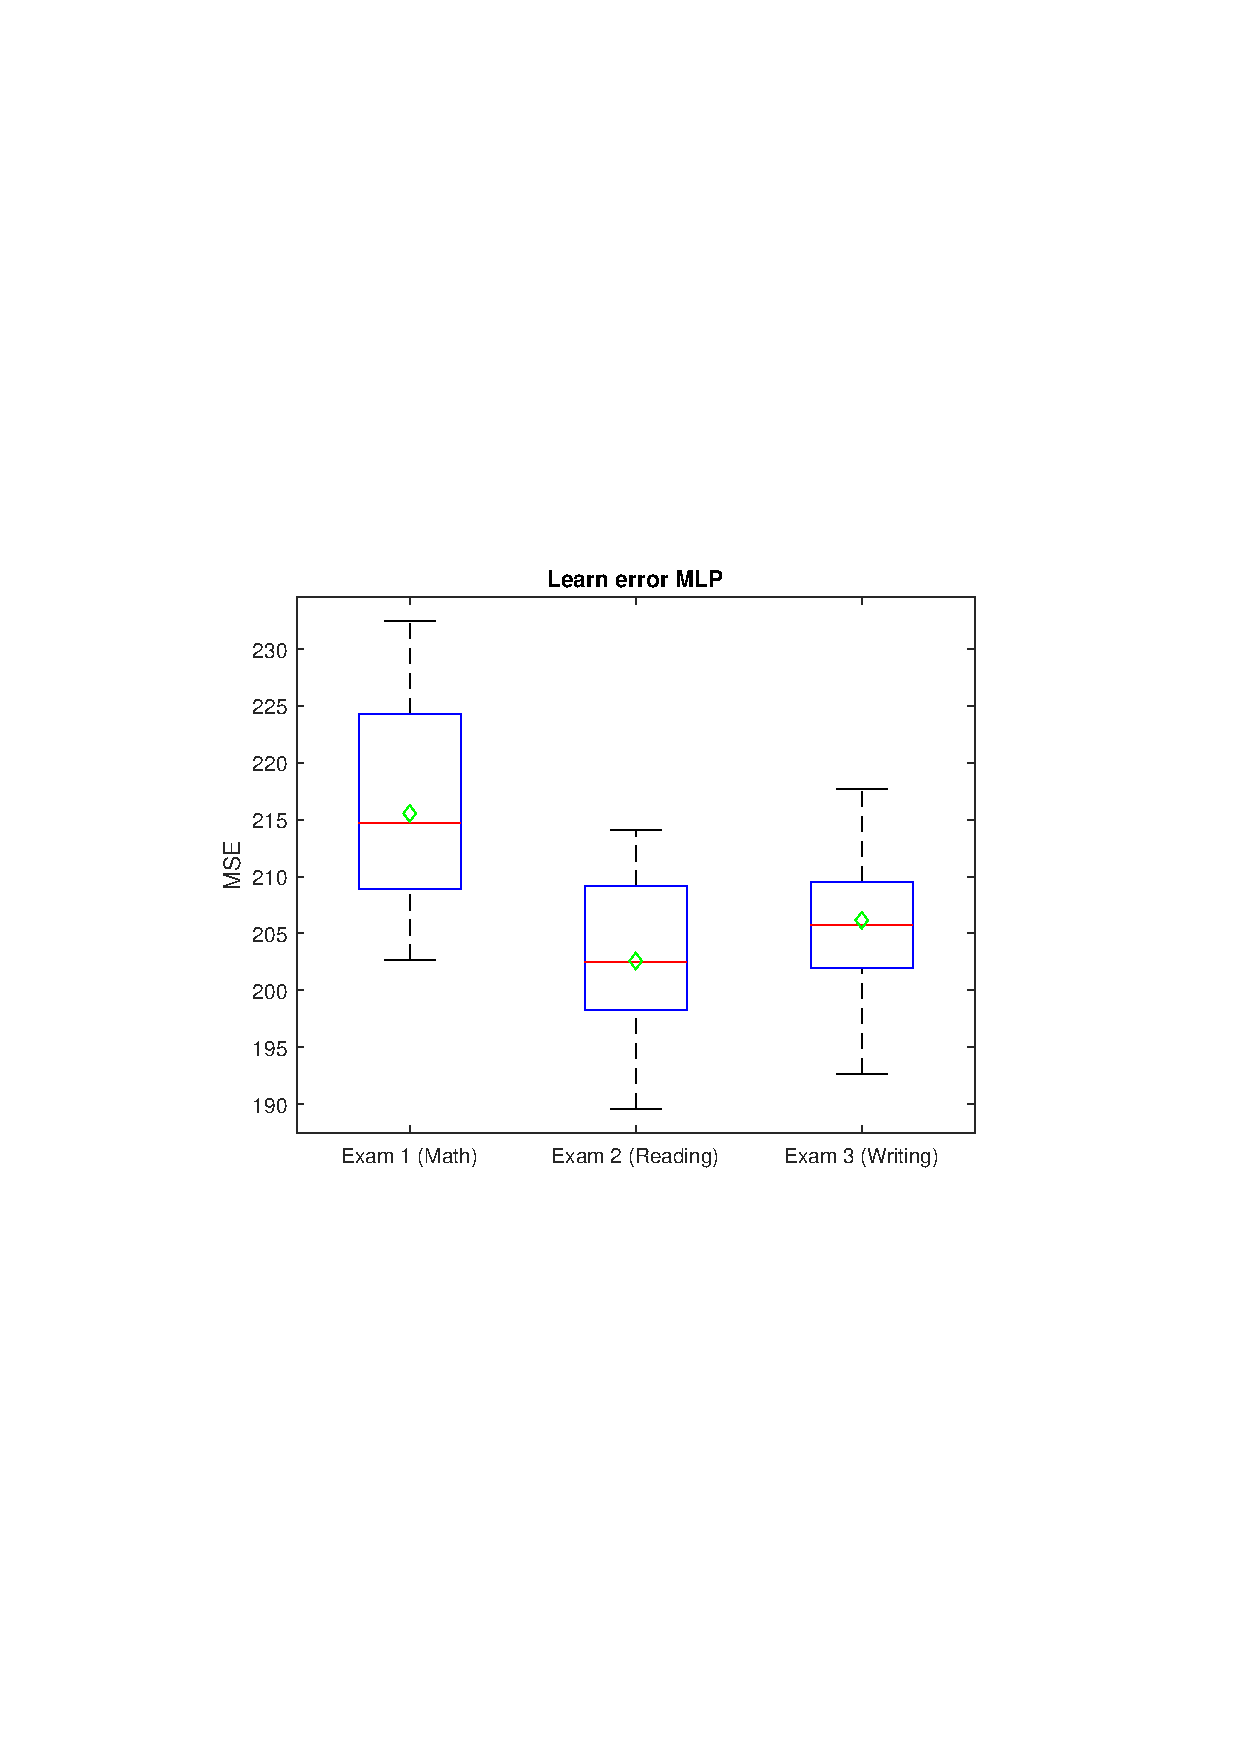
\includegraphics[height=3.3in]{purelin_purelin_20_without_4_learnBoxplot.pdf}
\caption{MSE uczenia dla  20 neuronów w pierwszej warstwie.}
\end{subfigure}
~~
\begin{subfigure}[t]{0.48\textwidth} 
\centering
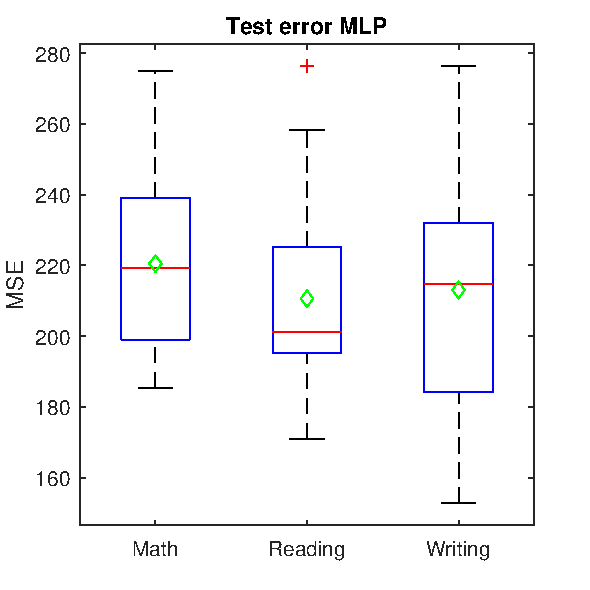
\includegraphics[height=3.3in]{purelin_purelin_20_without_4_testBoxplot.pdf}
\caption{MSE testu dla  20  neuronów w pierwszej warstwiej.}
\end{subfigure}

\caption{Błąd uczenia i testowania sieci w przypadku usunięcia czwartej  kolumny z danymi, \textbf{funkcje: purelin, purelin}.}
\end{figure}


\subsection{Uzyskane błędy w przypadku usunięcia piątej kolumny}
Jako ostatnia ze zbioru uczącego została usunięta kolumna informująca o ukończeniu kursu przygotowawczego. Otrzymane wyniki przedstawiono poniżej.
\begin{figure}[H]
\centering
\begin{subfigure}[t]{0.48\textwidth} 
\centering
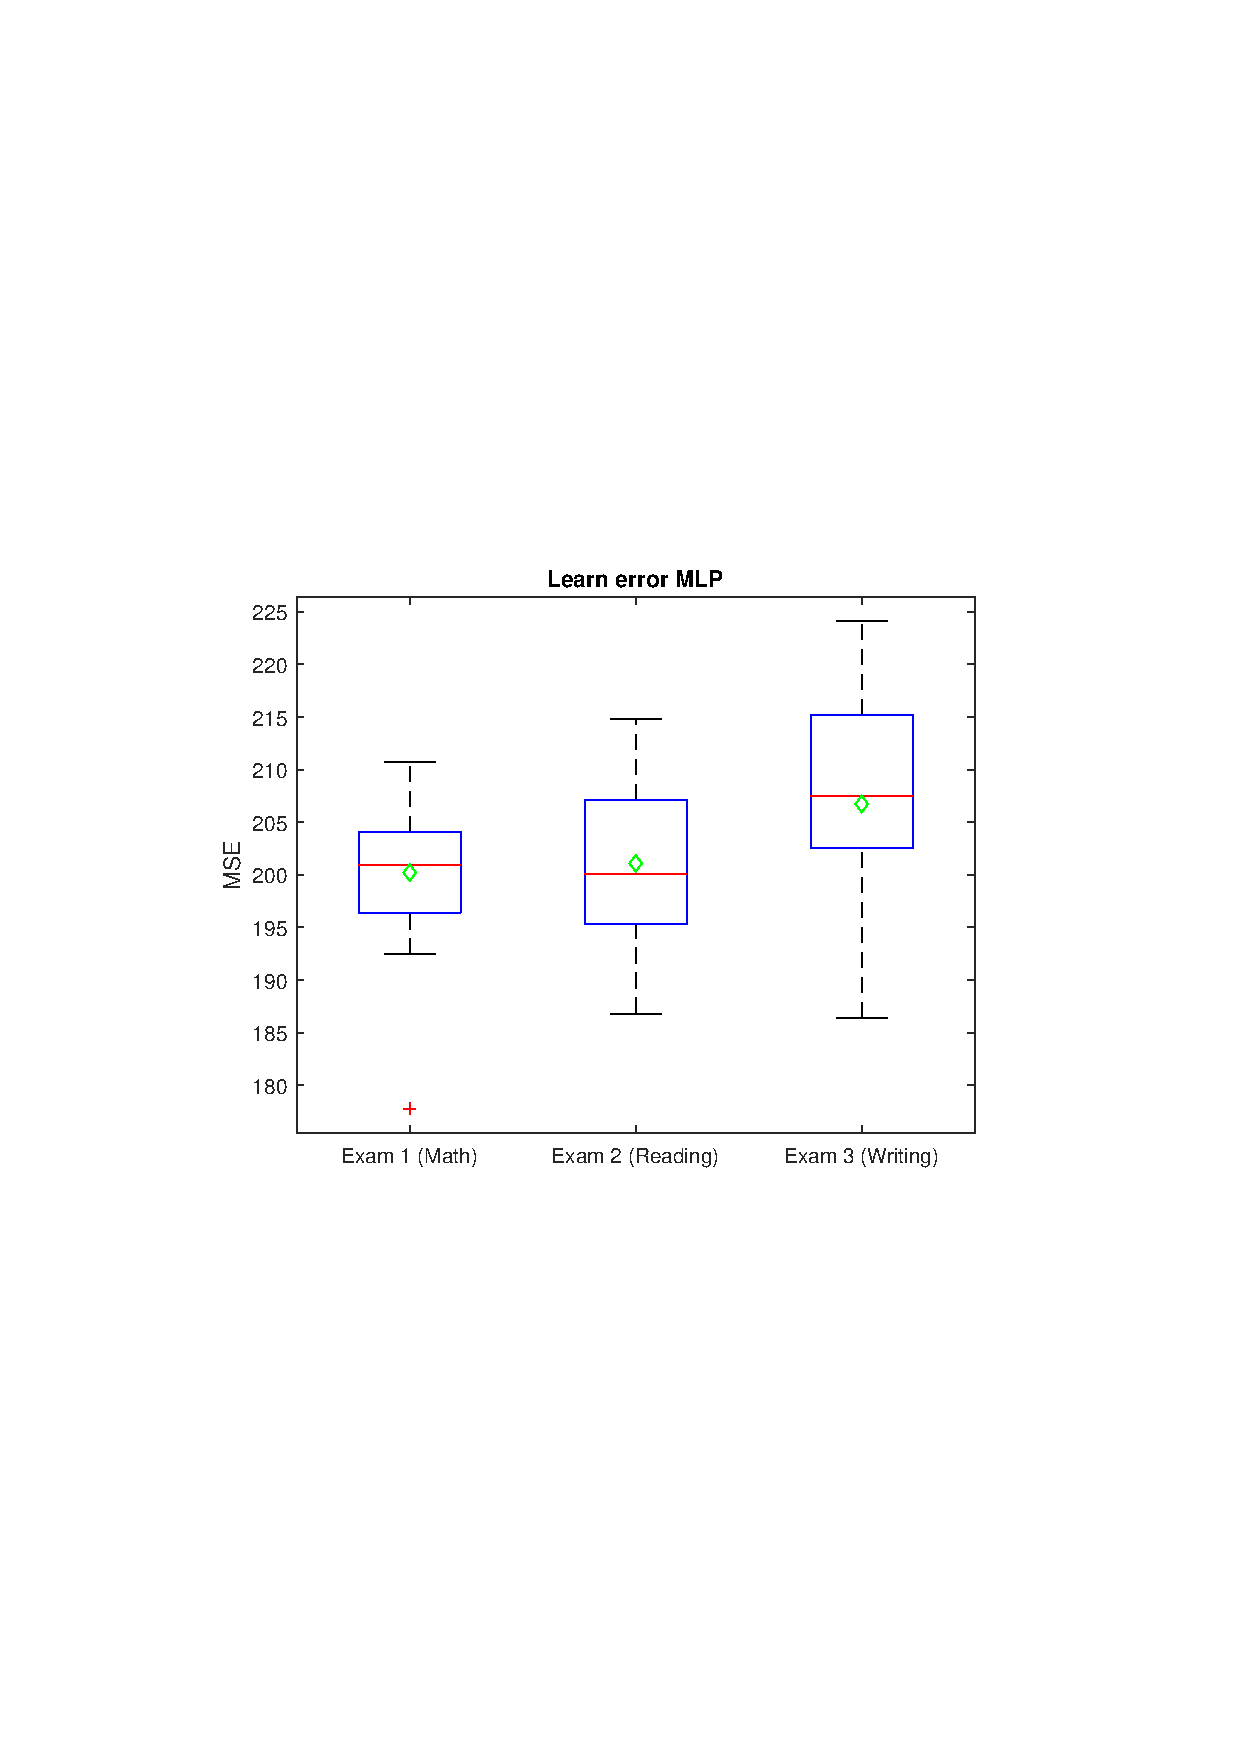
\includegraphics[height=3.3in]{purelin_purelin_20_without_5_learnBoxplot.pdf}
\caption{MSE uczenia dla  20 neuronów w pierwszej warstwie.}
\end{subfigure}
~~
\begin{subfigure}[t]{0.48\textwidth} 
\centering
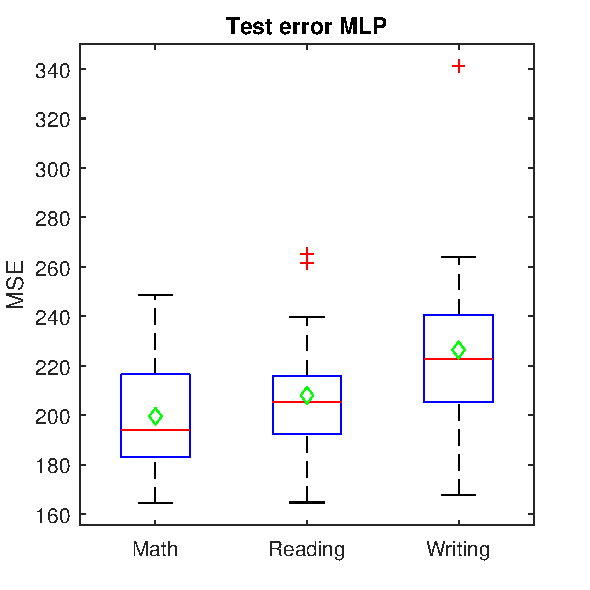
\includegraphics[height=3.3in]{purelin_purelin_20_without_5_testBoxplot.pdf}
\caption{MSE testu dla  20  neuronów w pierwszej warstwiej.}
\end{subfigure}

\caption{Błąd uczenia i testowania sieci w przypadku usunięcia piątej  kolumny z danymi, \textbf{funkcje: purelin, purelin}.}
\end{figure}


\subsection{Wnioski}
Badano wersję z funkcjami purelin, purelin oraz 20 neuronami w pierwszej warstwie.
% Wnioski do dopisania

\pagebreak
\section{Przewidywanie wyniku egzaminu bazując na rezultatach pozostałych egzaminów}
Jak zostało zauważone podczas badania korelacji, wyniki egzaminów są od siebie zależne (wysoki współczynnik korelacji). Korzystając z wyników z dwóch egzaminów podjęto próbę stworzenia sieci obliczającą wynik z trzeciego egzaminu. Sieć została skonfigurowana według najlepszych znalezionych parametrów.

Otrzymane błędy testowania zostały przedstawione poniżej.

\begin{figure}[H]
\centering
\begin{subfigure}[t]{0.48\textwidth} 
\centering
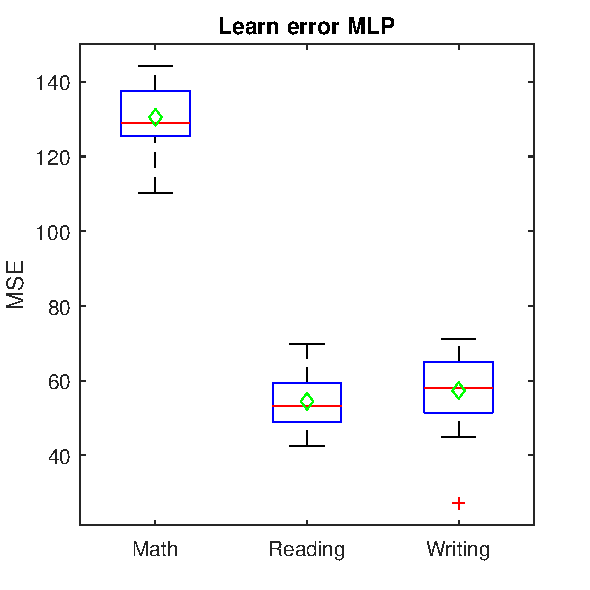
\includegraphics[height=3.3in]{cz3_egz_learn.pdf}
\caption{MSE uczenia dla 20 prób, dla kolejnych egzaminów.}
\end{subfigure}
~~
\begin{subfigure}[t]{0.48\textwidth} 
\centering
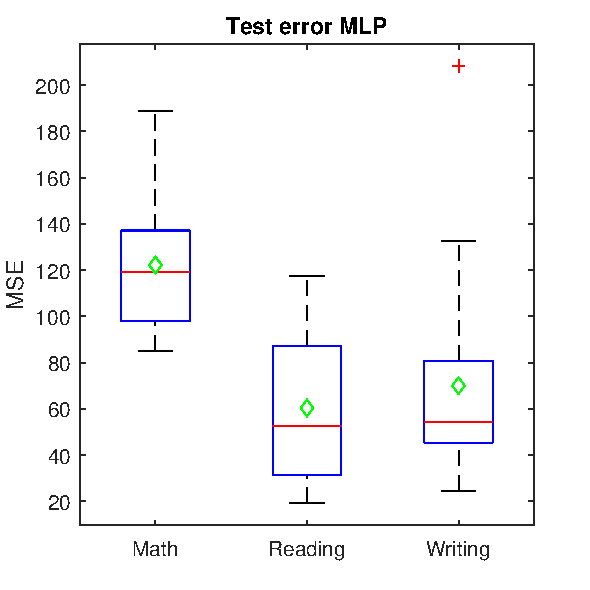
\includegraphics[height=3.3in]{cz3_egz_test.pdf}
\caption{MSE testowania dla 20 prób, dla kolejnych egzaminów.}
\end{subfigure}
\end{figure}

Na podstawie obserwacji wielkości błędów, można zauważyć, że dla egzaminów 2 oraz 3 sieć osiąga dobre wyniki - na poziomie wartości $50$.  Są one o wiele niższe niż dla sieci uczonej czynnikami środowiskowymi.

Otrzymane wyniki można powiązać z analizowaną wcześniej korelacją danych - wyniki egzaminów 2 i 3 są ze sobą w większym stopniu powiązane, niż egzamin 1 z egzaminem 2 lub 3.

Na rysunkach poniżej został przedstawiony za pomocą histogramu rozkład błędów, postały przy pojedynczym uruchomieniu. Za każdym razem histogramy te różniły się między sobą lecz zaobserwowane tendencje pozostawały takie same.

\begin{figure}[H]
\centering
\begin{subfigure}[t]{0.48\textwidth} 
\centering
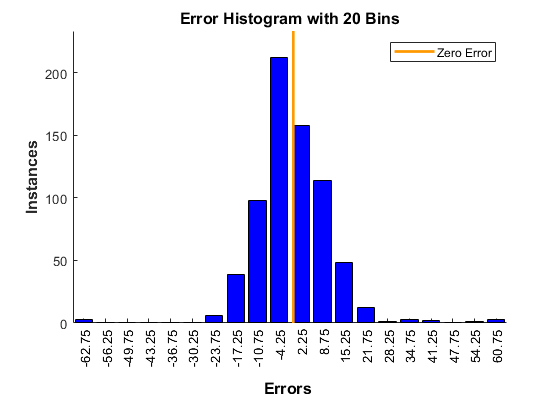
\includegraphics[width=\textwidth]{hist_exam_1_learn.png}
\caption{Rozkład błędów dla zbioru uczącego dla egzaminu 1 (matematyka).}
\end{subfigure}
~~
\begin{subfigure}[t]{0.48\textwidth} 
\centering
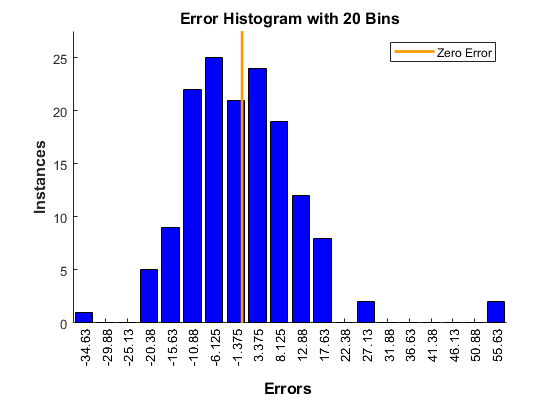
\includegraphics[width=\textwidth]{hist_exam_1_test.png}
\caption{Rozkład błędów dla zbioru testującego dla egzaminu 1 (matematyka).}
\end{subfigure}

\centering
\begin{subfigure}[t]{0.48\textwidth} 
\centering
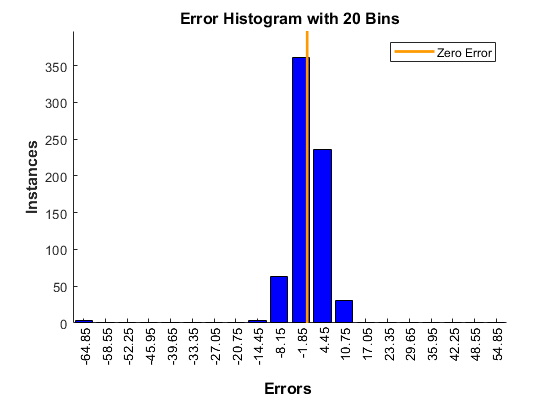
\includegraphics[width=\textwidth]{hist_exam_2_learn.png}
\caption{Rozkład błędów dla zbioru uczącego dla egzaminu 2  (czytanie).}
\end{subfigure}
~~
\begin{subfigure}[t]{0.48\textwidth} 
\centering
\includegraphics[width=\textwidth]{hist_exam_2_test.png}
\caption{Rozkład błędów dla zbioru testującego dla egzaminu 2  (czytanie).}
\end{subfigure}

\centering
\begin{subfigure}[t]{0.48\textwidth} 
\centering
\includegraphics[width=\textwidth]{hist_exam_3_learn.png}
\caption{Rozkład błędów dla zbioru uczącego dla egzaminu 3 (pisanie).}
\end{subfigure}
~~
\begin{subfigure}[t]{0.48\textwidth} 
\centering
\includegraphics[width=\textwidth]{hist_exam_3_test.png}
\caption{Rozkład błędów dla zbioru testującego dla egzaminu 3 (pisanie).}
\end{subfigure}
\end{figure}

Największa ilość błędów we wszystkich przypadkach to te bliskie zeru. Przy testowaniu zbioru uczącego wartości są bardziej skoncentrowane, szczególnie dla egzaminów 2 oraz 3. Chociaż różnica pomiędzy wartością oczekiwaną a doświadczalną jest czasem duża, sieć w większości przypadków potrafi przewidzieć wynik egzaminu z dokładnością do 10 punktów. 

\pagebreak
\section{Podsumowanie}


W przypadku uczenia sieci wynikami egzaminów, jakość jej działania jest o wiele wyższa niż w przypadku uczenia jej czynnikami środowiskowymi. Powiązane jest to z faktem, że korelacja pomiędzy kolumnami z wynikami egzaminów jest o wiele większa niż pomiędzy egzaminami a czynnikami środowiskowymi. Jednak, gdy chcielibyśmy użyć sieci w prawdziwym życiu, przed egzaminami nie dysponujemy taką wiedzą. Można by było posłużyć się wynikami egzaminów próbnych - jednak jako że nie były one zawarte w naszym zbiorze, więc ta hipoteza musiałaby zostać zbadana.

Oprócz wyników egzaminu, duży wpływ ma ukończenie kursu przygotowawczego - szczególnie z matematyki. Usunięcie tej kolumny pomniejszyło jakość działania sieci. Dla pozostałych dwóch zbiorów podobnie duży wpływ ma jeszcze płeć oraz dieta studenta.

W żadnej konfiguracji nie udało nam się uzyskać bardzo dobrych wyników, co można uznać za pozytywną informację dla studentów. Ich wyniki nie są zdeterminowane rasą, płcią czy rezultatami pozostałych egzaminów, a ich realną pracą i wysiłkiem włożonym w przygotowanie (choć samo ukończenie kursu nie ma bardzo dużego znaczenia). Do stworzenia idealnej sieci potrzebna by była większa ilość danych, na przykład na temat samodzielnej pracy studenta, czy wyników egzaminów próbnych. 

Gdy przyjmiemy, że nasza sieć powinna znajdować wynik w granicach błędu np 5 punktów (na 100 wszystkich możliwych) jakość wyników sieci wzrasta. 

\pagebreak

\begin{thebibliography}{9}

\bibitem{kaggle-student}
Zbiór danych  \textit{Students Performance in Exams} - \url{https://www.kaggle.com/spscientist/students-performance-in-exams}

\bibitem{kaggle}
Platforma \textit{Kaggle} - \url{https://www.kaggle.com/}

\bibitem{wiki}
Perceptron wielowarstwowy - \url{https://pl.wikipedia.org/wiki/Perceptron_wielowarstwowy}

\bibitem{mlp-schema}
ASSESSMENT OF ARTIFICIAL NEURAL NETWORK FOR BATHYMETRY ESTIMATION USING HIGH RESOLUTION SATELLITE IMAGERY IN SHALLOW LAKES: CASE STUDY EL BURULLUS LAKE. - \url{https://www.researchgate.net/publication/303875065_ASSESSMENT_OF_ARTIFICIAL_NEURAL_NETWORK_FOR_BATHYMETRY_ESTIMATION_USING_HIGH_RESOLUTION_SATELLITE_IMAGERY_IN_SHALLOW_LAKES_CASE_STUDY_EL_BURULLUS_LAKE}

\end{thebibliography}

\end{document}